\documentclass[11pt, a4paper, oneside]{book}

\usepackage{fancyhdr}
\pagestyle{fancy}
\fancyhf{}

\usepackage[english]{babel}
\usepackage{graphicx}
\usepackage[colorlinks,hyperindex,plainpages=false,breaklinks]{hyperref}
\usepackage{amssymb}
\usepackage{wasysym} 
\usepackage{wrapfig}
\usepackage{enumerate}
\usepackage{placeins} % Necessary for \FloatBarrier
\usepackage{subfig}   % Necessary for subfloat (images next to each other)
\usepackage{color}
\usepackage[usenames,dvipsnames,svgnames]{xcolor}
\usepackage{listings}

\definecolor{codelightgray}{rgb}{0.87,0.87,0.87}

\hypersetup{colorlinks=true,% 
	linkcolor=black,%
	citecolor=red,%
	filecolor=blue,% 
	menucolor=black,% 
	pagecolor=black,%
	urlcolor=black}
	
\lstset{language=,
    keywordstyle=\color{blue},
    basicstyle=\scriptsize\ttfamily,
    showstringspaces=false,
    backgroundcolor=\color{codelightgray},
    morekeywords={SELECT,FROM,WHERE,AND,OR,EClass}
}

\newcommand{\note}[1]{\marginpar{\emph{#1}}}

\setcounter{tocdepth}{3}

\setlength{\parindent}{0pt} 
\setlength{\parskip}{0.3cm}

\graphicspath{%
{../../00_introduction/common/}%
{../2_staticSemantics/vis_anAbstractDefinition/abstractImages/}{../2_staticSemantics/tex_ConcreteDefinition/concreteImages/}%
{../3_validatingMetamodel/vis_EAValidation/03_images/}%
{../4_creatingInstance/04_images/}%
}

% Remove section numbers 0.1, 0.2 ..
\renewcommand{\thesection}{\arabic{section}} 

% --- Title Page Information --------------------------------------------------------
\def\partTitle{Part II: Leitner's Learning Box}
\def\versionNumber{0.5}
\title{
\flushright
{\LARGE\bfseries An Introduction to Metamodelling\\
and Graph Transformations}
\noindent\rule[-1ex]{\textwidth}{5pt}\\[2.5ex]
\hfill\emph{\LARGE\bfseries with eMoflon}
\flushleft
{\small Version 2.1}
\flushright

\includegraphics[width=0.85\textwidth]{pics/eMoflon3} 
}

\date{}  
\author{} 

% --- HEADER FUNCTIONS --------------------------------------------------------------
% Default plain header; turn off all lines and colors
\newcommand{\noHeader}{
	\fancyfoot{}
	% NOTE: since this is the first header, we effectively 'turn on' the page numbers. They don't need to be re-declared in each heading.
 	\fancyhead[R]{\thepage}
	\fancyhead[L]{}
	\renewcommand{\headrulewidth}{0pt}
}

% Common Header, Black
\newcommand{\genHeader}{
	\fancyfoot{}
	\fancyhead[L]{}
	\renewcommand{\headrulewidth}{1.5pt}
 	\renewcommand{\headrule}{\hbox to\headwidth{%
  		\color{Black}\leaders\hrule height \headrulewidth\hfill}}
}

% Visual instructions only, Red header
\newcommand{\visHeader}{
	\fancyfoot{}
	\fancyhead[L]{\color{RedOrange}\tiny \bf VISUAL}
	\renewcommand{\headrulewidth}{1.5pt}
	\renewcommand{\headrule}{\hbox to\headwidth{%
  		\color{RedOrange}\leaders\hrule height \headrulewidth\hfill}}
}

% Text instructions only, Blue header
\newcommand{\texHeader}{
	\fancyfoot{}
	\fancyhead[L]{\color{ProcessBlue}\tiny \bf TEXTUAL}
	\renewcommand{\headrulewidth}{1.5pt}
	\renewcommand{\headrule}{\hbox to\headwidth{%
  		\color{ProcessBlue}\leaders\hrule height \headrulewidth\hfill}}
}

% ---------------------------------------------------------------------------------

\begin{document}

\frontmatter 
\noHeader

% Title Page without blank
{\let\newpage\relax\maketitle}

% Copyright notice
\begin{small} 
Copyright \copyright~2011--\the\year{} Real-Time Systems Lab, TU Darmstadt.
Anthony Anjorin, Erika Burdon, Frederik Deckwerth, Roland Kluge, Marius Lauder,
Erhan Leblebici, Daniel T\"ogel, David Marx, Lars Patzina, Sven Patzina, Alexander Schleich, Sascha Edwin Zander, Jerome Reinl\"ander, Martin Wieber, and contributors.
All rights reserved.

This document is free; you can redistribute it and/or modify it under the terms of the GNU Free Documentation License as published by the Free Software Foundation; either version 1.3 of the License, or (at your option) any later version.
Please visit \href{http://www.gnu.org/copyleft/fdl.html}{http://www.gnu.org/copyleft/fdl.html} to find the full text of the license.
 
% TODO Remove this?? It can be found easily online .. (we can even offer it on
% the download page) For your convenience, this document includes a copy of the \emph{GNU General Public License} starting from page~\pageref{chap:gpl}.
  
For further information contact us at \eMoflonContact.
  
\vskip3cm
\textit{The eMoflon team}\\
Darmstadt, Germany (\monthword{\month} \the\year)
\end{small}
\let\cleardoublepage\clearpage

% TOC
\tableofcontents

% Store page counter
\newcounter{romanpages}
\setcounter{romanpages}{\value{page}}

\mainmatter

% Main content for this Part
\part{\partTitle}
\label{chap:ecore}

\genHeader

The toughest part of learning a new language  is often building up a sufficient vocabulary.
This is usually accomplished by repeating a long list of words again and again till they stick.
A \emph{Leitner's learning box}\footnote{http://en.wikipedia.org/wiki/Leitner\_system} is a simple but ingenious little contraption to support this tedious process of memorization.

As depicted in Fig.~\ref{fig:membox_illustration}, it consists of a series of compartments or partitions usually of increasing size.
The content to be memorized is written on a series of cards  which are initially placed in the first partition.
All cards in the first  partition should be repeated everyday and cards that have been successfully memorized are placed in the next partition.
Cards in all other partitions are only repeated when the corresponding partition is full and cards that are  answered correctly are moved one partition forward in the box.
Challenging  cards that have been forgotten are treated as brand new cards and are always  placed right back into the first partition regardless of how far in the box they  had progressed.

These ``rules'' are depicted by the green and red arrows in  Fig.~\ref{fig:membox_illustration}.
The basic idea is to repeat difficult cards as often as necessary and not to waste time on easy cards which
are only repeated now and then to keep them in memory.
The increasing size of the partitions represents how words are easily placed in our limited short term memory and slowly move in our theoretically unlimited long term memory if practised often enough.

%\usepackage{graphics} is needed for \includegraphics
 \begin{figure}[htp]
 \begin{center}
   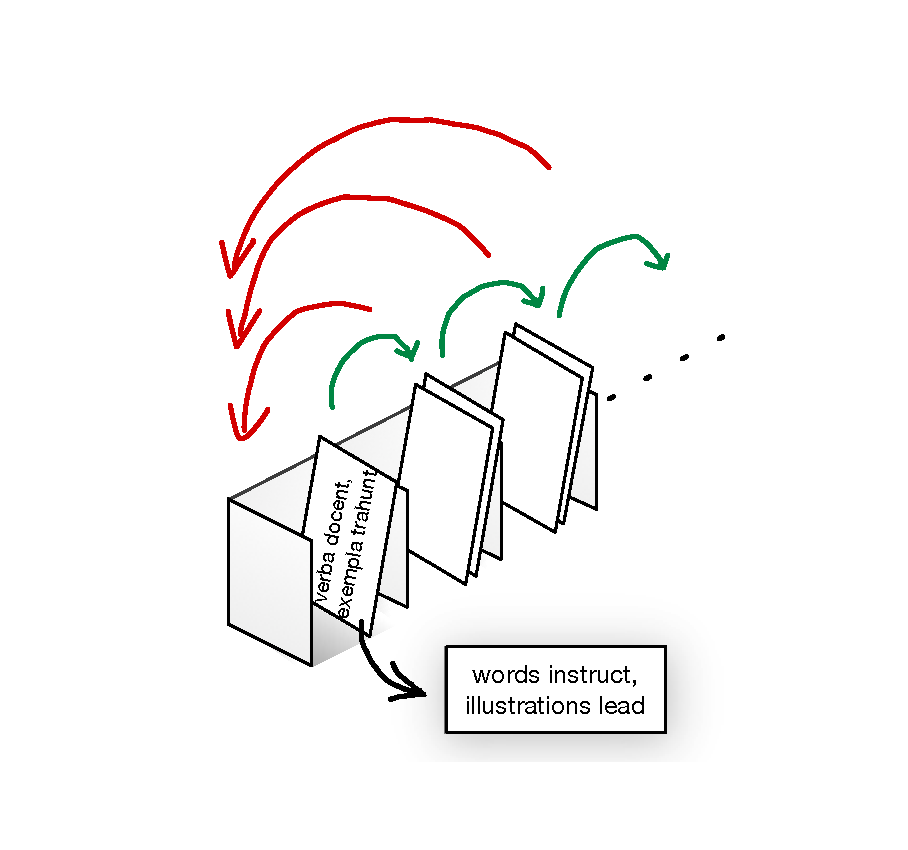
\includegraphics[width=0.5\textwidth]{../membox_illustration}
   \caption[]{Possible \emph{Concrete Syntax} of a Leitner's Learning Box.}
   \label{fig:membox_illustration}
 \end{center}
 \end{figure}
 \FloatBarrier

A learning box is an interesting system, because it consists clearly of a static structure (the box, partitions and their sizes, cards with their sides and corresponding content) and a set of rules that describe the dynamic aspects
(behaviour) of the system.
In the rest of the tutorial we shall build a complete learning box from scratch in a model-driven fashion and use it to introduce fundamental concepts in metamodelling and \emph{Model-Driven Software Development} (MDSD) in general.



\section{A language definition problem?}

% START BUILDING GLOSSARY HERE? http://tex.stackexchange.com/questions/34641/which-tool-to-use-an-index-or-a-glossary
As in any area of study, metamodelling has its fair share of buzz words used by experts to communicate concisely.  Although some concepts might seem quite abstract for a beginner, a well defined vocabulary is important so we know
exactly what we are talking about.

The first step is understanding that metamodelling equates to language definition.
This means that the task of building a system like our learning box can be viewed as defining a suitable language that can be used to describe the system.
This language oriented approach has a lot of advantages including a natural support for product lines (individual products are valid members of the language) and a clear separation between platform independent and platform specific details.

So what constitutes a language?  The first question is obviously  how the building blocks of your language actually ``look'' like.
Is your language to be textual?  Visual?  This is referred to as the %line break for eay glossary testing 
\emph{Concrete Syntax} 
of a language and is basically an interface to end users who use the language.
\marginpar{\emph{Concrete Syntax}}
In the case of our learning box, Fig.~\ref{fig:membox_illustration} can be viewed as a possible concrete syntax.
As we are however building a learning box as a software system, our actual concrete syntax  will probably be composed of GUI elements like buttons, drop-down menus and text fields.

Irrespective of how a language looks like, members of the language must adhere to the same set of ``rules''.
\marginpar{\emph{Grammar}}
For a natural language like English, this set of rules is usually called a \emph{grammar}.
In metamodelling, however, everything is represented as a graph of some kind and, although the concept of a  \emph{graph grammar} is also quite well-spread and understood, metamodellers  more often use a \emph{type graph} that defines what types and relations  constitute a language.
\marginpar{\emph{Graph Grammar}}
\marginpar{\emph{Type Graph}}
A graph that is a member of your language must \emph{conform to} the corresponding type graph for the language.
To be more precise, it must be possible to type the graph according to the type graph, i.e., the types and relations used in the graph must exist in the type graph and not contradict the structure defined there.
\marginpar{\emph{Abstract Syntax}}
This way of defining membership to a language has many parallels to the class-object relationship in the object-oriented paradigm and should seem very familiar for any programmer used to OO.
This type graph is referred to as the \emph{Abstract Syntax} of a language.

Very often, one might want to further constrain a language, beyond simple typing rules.
\marginpar{\emph{Static Semantics}}
This can be accomplished with a further set of rules or constraints that members of the language must fulfil in addition to being conform to the type graph.
These further constraints are referred to as the \emph{Static Semantics} of a language.

With these few basic concepts, we can now introduce a further and central concept in metamodelling, the \emph{metamodel} (basically a simple class diagram).
\marginpar{\emph{Metamodel}}
A metamodel defines not only the abstract syntax of a language but also some basic constraints (a part of the static semantics).
Thinking back to our learning box, we could define the types and relations we want to allow, e.g.,  a box with partitions, cards, the box contains partitions that contain cards.
Multiplicities are an example for constraints that are no longer part of the abstract syntax and belong to static semantics, but can nonetheless be expressed in a metamodel.
For example, that a card can only be in one partition, or that a partition has only one next partition or none.
\marginpar{\emph{Constraint Language}}
More complex constraints that cannot be expressed in a metamodel are usually specified using an extra \emph{constraint language} such as OCL (the Object Constraint Language).
This goes beyond this tutorial however and we'll stick to metamodels without using an extra constraint language.

$\textbf{A short recap:}$  we have learnt that metamodelling starts with defining a suitable language.
For the moment, we know that a language comprises a concrete syntax (how does the language look like),  an abstract syntax (types and relations of the underlying graph structure), and static semantics (further constraints that members of the language must fulfil).
Metamodels are used to define the abstract syntax and a part of the static semantics of a language, while \emph{models} are graphs that conform to some
\marginpar{\emph{Model}}
metamodel (can be typed  according to the abstract syntax and adhere to the static semantics).

This tutorial is meant to be be hands-on so enough theory!
Lets define, step-by-step, a metamodel for our learning box using our tool eMoflon.

\newpage
\section{Abstract syntax and static semantics}
\label{sec: staticSemantics}

Introduction to the section starts here (to avoid hopping right into a subsection). ((looks ugly!))
Explain order of operations (for a new metamodel)? New start, define classes, create references, create methods.

\newpage
\subsection{Getting started in EA}
\visHeader
\hypertarget{static:starting vis}{}
  
{\bf Note:} To continue with Part I's Demo files, open the \texttt{demo.eap} file in EA, initialise a new diagram, then work within that EA project. You can
ignore the first instruction below. (test this!)

\begin{itemize}

\item[$\blacktriangleright$]  To begin, navigate to ``New Metamodel Project,'' and start a new visual project (this time without the demo specifications)
named \texttt{Leit\-ners\-Learn\-ing\-Box} (Fig.~\ref{fig:new_visModel}). Open the empty \texttt{.eap} file in EA.

\vspace{0.5cm}

\begin{figure}[htbp]
	\centering
  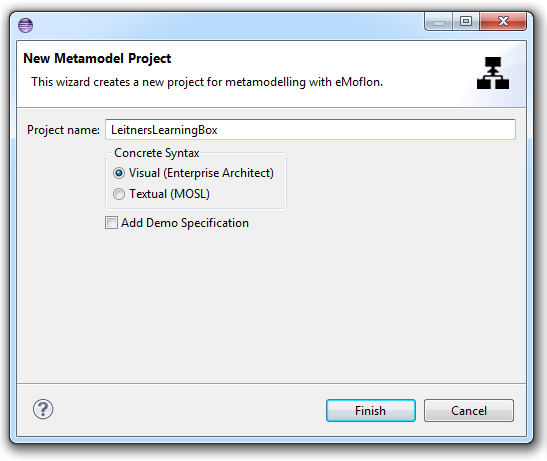
\includegraphics[width=0.8\textwidth]{eclipse_visNewMetamodelPlain}
	\caption{Starting a new visual project}
	\label{fig:new_visModel}
\end{figure}

\vspace{0.5cm}

\item[$\blacktriangleright$] In EA, select your working set and press the ``Add a Package'' button (Fig.~\ref{fig:new_package}). (test: make sure
\texttt{eMoflonLanguages} is included in BOTH new file and Demo specs. (gotta look the same!) )

\begin{figure}[htbp]
	\centering
  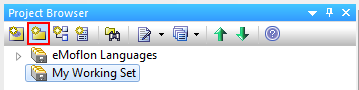
\includegraphics[width=0.5\textwidth]{ea_addPackage}
	\caption{Add a new package to \texttt{MyWorkingSet}}
	\label{fig:new_package}
	\vspace{0.5cm}
\end{figure}

\clearpage

\item[$\blacktriangleright$] In the dialogue that pops up (Fig.~\ref{fig:new_package_name}), enter \texttt{LearningBoxLanguage} as the name of the new
package. Make sure \texttt{Class View} is selected, and click \texttt{OK}.

\vspace{0.5cm}

\begin{figure}[htbp]
	\centering
    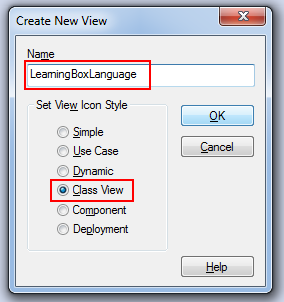
\includegraphics[width=0.33\textwidth]{ea_nameEPackage.png}
	\caption{Enter the name of the new package}
	\label{fig:new_package_name}
\end{figure}
\FloatBarrier

\vspace{0.5cm}

\item[$\blacktriangleright$] Your \texttt{Project Browser} should now resemble Fig.~\ref{fig:new_package_completed}.

\vspace{0.5cm}

\begin{figure}[htbp]
	\centering
  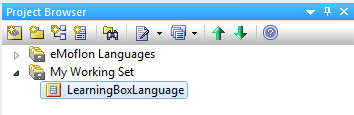
\includegraphics[width=0.5\textwidth]{ea_newPackage}
	\caption{State after creating the new package.}
	\label{fig:new_package_completed}
\end{figure}
\FloatBarrier


\vspace{0.5cm}

\item[$\blacktriangleright$] Now select your package and create a ``New Diagram'' (Fig.~\ref{fig:diagram}).

\vspace{0.5cm}

\begin{figure}[htbp]
	\centering
  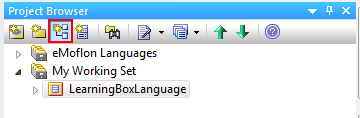
\includegraphics[width=0.5\textwidth]{ea_addDiagram}
	\caption{Add a diagram.}
	\label{fig:diagram}
\end{figure}
\FloatBarrier

\clearpage

\item[$\blacktriangleright$] In the dialogue that appears (Fig.~\ref{fig:diagram_type}), choose \texttt{eMoflon Ecore Diagrams} and press \texttt{OK}. 

\begin{figure}[htbp]
	\centering
  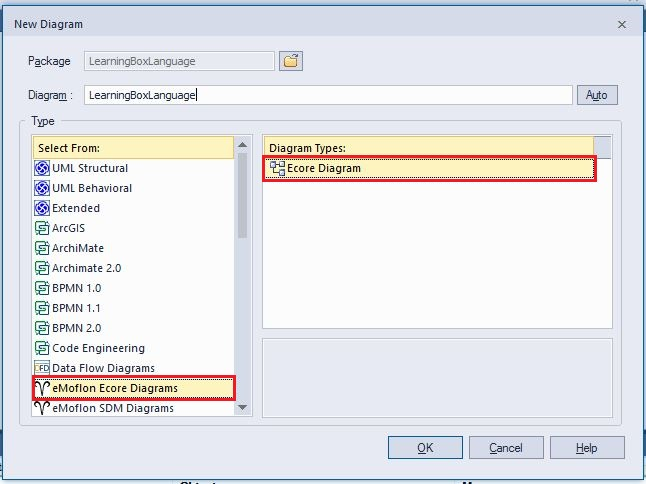
\includegraphics[width=0.8\textwidth]{ea_chooseDiagramType}
	\caption{Select the ecore diagram type}
	\label{fig:diagram_type}
\end{figure}
\FloatBarrier

 
\item[$\blacktriangleright$] After creating the new diagram, your  \texttt{Project Browser} should now resemble Fig.~\ref{fig:diagram_completed}. You'll notice
that your \texttt{LearningBoxLanguage} package has been transformed into an EPackage.

\begin{figure}[htbp]
	\centering
  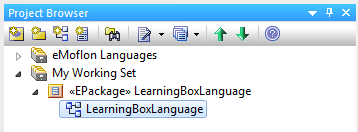
\includegraphics[width=0.5\textwidth]{ea_afterDiagramState}
	\caption{State after creating diagram}
	\label{fig:diagram_completed}
\end{figure}
\FloatBarrier

\item[$\blacktriangleright$] You can now already export your project to Eclipse,\footnote{If unsure how to perform this step, please
refer to Part I, section 2.1} then refresh your \texttt{Package Explorer}. A new node, \texttt{My Working Set}\footnote{If you do not have the two
distinct nodes, make sure your ``Top Level Elements'' are set to \texttt{Working Sets}} should have appeared containing your \texttt{Epackage}
(Fig.~\ref{fig:init_export}). You can see that a \texttt{LearningBoxLanguage.ecore} file has been generated, and placed in ``model.'' This is your metamodel
that will contain all future types you create in your diagrams.

\clearpage

\vspace*{2cm}

\begin{figure}[htbp]
	\centering
  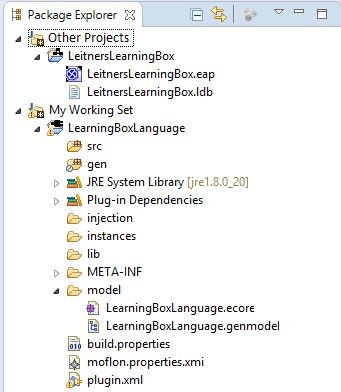
\includegraphics[width=0.55\textwidth]{eclipse_visInitExport}
	\caption{Inital export to Eclipse}
	\label{fig:init_export}
\end{figure}

\vspace{1cm}

\item[$\blacktriangleright$] If you're interested in reviewing the overall project structure, the purposes of certain files and folders, read section 4.1 from
Part~I\footnote{Download link: \dlPartOne} of this handbook. Otherwise, continue to the next to section learn how to declare classes and attributes.

\fancyfoot[R]{$\triangleright$ \hyperlink{static:classes vis}{Next}}
\end{itemize}

\clearpage
\subsection{Getting started with MOSL}
\texHeader
\hypertarget{static:starting tex}{} 

\begin{itemize}

\item[$\blacktriangleright$] Create a new metamodel project in Eclipse by navigating to the \texttt{New Metamodel} button in the toolbar. In the dialogue that
appears, enter \texttt{LeitnersLearningBox} as the project name, and select \texttt{Textual (MOSL)}  (Fig.~\ref{eclipse:newProject}).

\vspace{1cm}

\begin{figure}[htbp]
	\centering
  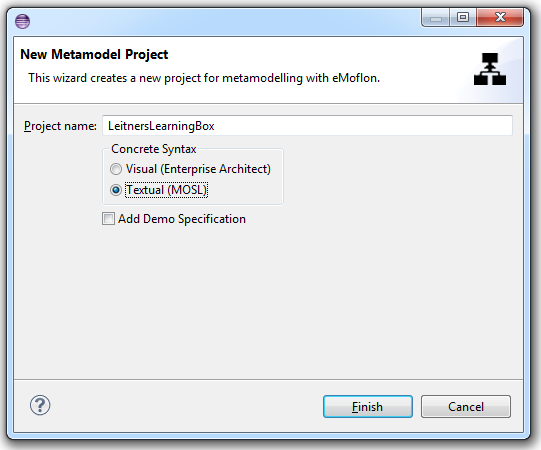
\includegraphics[width=0.8\textwidth]{eclipse_texNewMetamodelPlain}
	\caption{Creating a new metamodel project}
	\label{eclipse:newProject}
\end{figure}

\vspace{1cm}

\item[$\blacktriangleright$] You'll see your new project appear under the ``Specifications" node.\footnote{If no nodes appear in your package explorer,
ensure your ``Top Level Elements'' are set to ``WorkingSets''} If you're interested in the details of eMoflon's project structure, review Section
4.2 from Part I. Otherwise, expand the project as deep as it goes (Fig.~\ref{eclipse:expandedFolders}).

\clearpage

\begin{figure}[htbp]
	\centering
  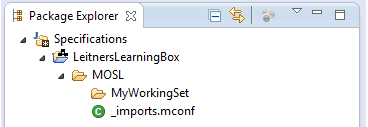
\includegraphics[width=0.6\textwidth]{eclipse_texFoldersExpanded}
	\caption{Expanded project files}
	\label{eclipse:expandedFolders}
\end{figure} 

\vspace{0.5cm}

\item[$\blacktriangleright$] We're most interested in \texttt{MOSL/MyWorkingSet}, which represents the project scope. Right click this folder, and create a new
\texttt{EPackage} (Fig.~\ref{eclipse:newEPackage}), naming it \texttt{LearningBoxLanguage}. Using this wizard to generate your EPackage will automatically
create the necessary \texttt{\_patterns} folder and \texttt{\_constraints} file.

\vspace{0.5cm}

\begin{figure}[htbp]
	\centering
  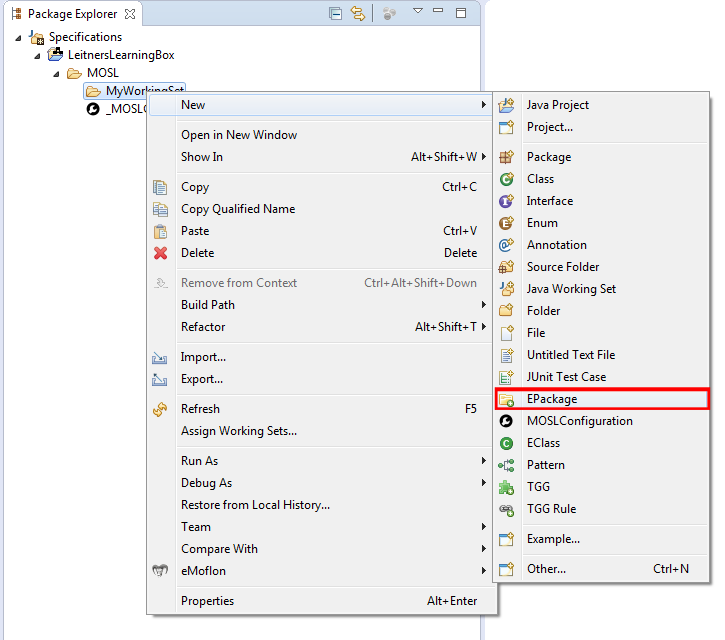
\includegraphics[width=0.8\textwidth]{eclipse_newEPackage}
	\caption{Create an EPackage in your working set}
	\label{eclipse:newEPackage}
\end{figure} 

\clearpage

\item[$\blacktriangleright$] Your package explorer should now resemble Fig.~\ref{eclipse:preBuild}.

\item[$\blacktriangleright$] To finish initalising your metamodel, navigate to ``Build (Without cleaning),'' found beside ``New Metamodel'' in the
toolbar (Fig.~\ref{eclipse:preBuild}).

\begin{figure}[htbp]
	\centering
  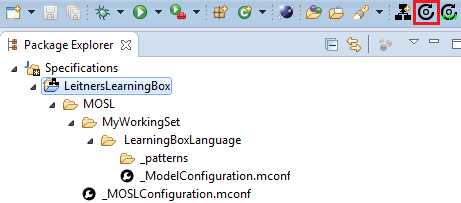
\includegraphics[width=0.6\textwidth]{eclipse_texBuildButton}
	\caption{Inital structure of Leitner's Learning Box}
	\label{eclipse:preBuild}
\end{figure} 

\vspace{0.5cm}

\item[$\blacktriangleright$] A new, ``MyWorkingSet'' node, named after your project container, should have been created (Fig.~\ref{eclipse:finalFiles}). The
folder ``gen'' is where all Java files generated from your metamodel will be placed.

\vspace{0.5cm}

% Forced position at the bottom of the page
\begin{figure}[h!]
	\centering
  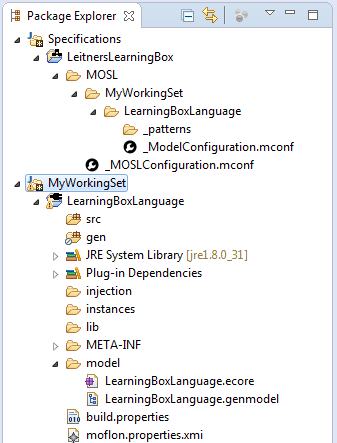
\includegraphics[width=0.5\textwidth]{eclipse_texFinalExpansion}
	\caption{The project fully initialised}
	\label{eclipse:finalFiles}
\end{figure} 

\vspace{0.5cm}

\item[$\blacktriangleright$] Navigate to ``LearningBoxLanguage/model.'' This folder contains \\ \texttt{LearningBoxLanguage.ecore}, your metamodel. This will
contain all types you define in ``LeitnersLearningBox/MOSL/MyWorkingSet/LearningBoxLanguage.''

\item[$\blacktriangleright$] Your project structure is now complete! In the next section, we'll start creating classes and attributes.

\jumpSingle{static:classes tex}

\end{itemize}


\newpage
\subsection{Declaring classes and attributes}
\genHeader
\hypertarget{static:classes vis}{}

\begin{stepbystep}

\item Return to EA, and double-click your \texttt{LearningBoxLanguage} diagram to ensure it's open.

\vspace{0.5cm}

\item There are two ways for you to create your first \texttt{EClass}. First, to the left of the workbench, a \emph{Toolbox} containing
the Ecore types available for metamodelling should have appeared (\Cref{ea:eclass}).\footnote{If not, choose ``Diagram/Diagram Toolbox'' to show the
current toolbox (Alt+ 5)} Click on the \texttt{EClass} icon then somewhere in the diagram to create a new object. Alternatively, you can click in the diagram and press
\texttt{space} to invoke the toolbox context menu, then select \texttt{EClass}.

\vspace{0.5cm}

\begin{figure}[htbp]
	\centering
  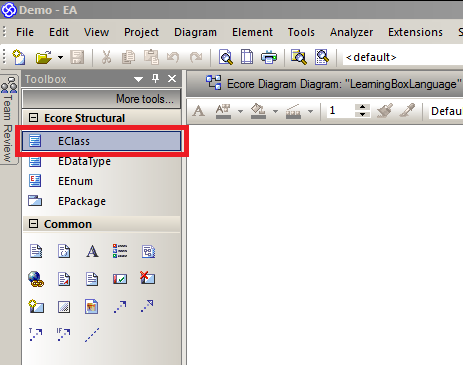
\includegraphics[width=0.7\textwidth]{ea_createEClass}
	\caption{Create an EClass}
	\label{ea:eclass}
\end{figure}

\vspace{0.5cm}

\item In the dialogue that pops-up, set \texttt{Box} as the name and click \texttt{OK} (\Cref{ea:eclass_properties}).
This dialogue can always be invoked again by double-clicking the EClass, or by pressing \texttt{Alt} and single-clicking. It contains many other properties that we'll investigate later in the handbook. In general, a similar properties dialogue can be opened in the same fashion for almost every element in EA.

\clearpage

\begin{figure}[ht]
	\centering
  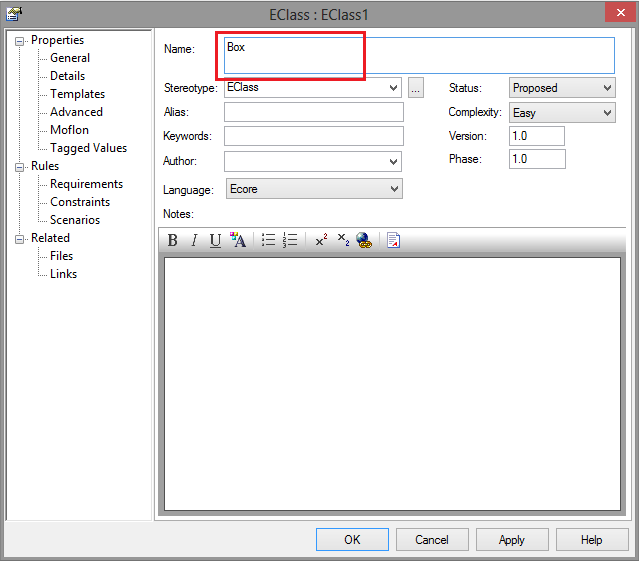
\includegraphics[width=0.9\textwidth]{ea_propertiesEClass}
	\caption{Edit the properties of an EClass}
	\label{ea:eclass_properties}
\end{figure}

\item After creating \texttt{Box}, your EA workspace should resemble \Cref{ea:eclass_completed}.

\vspace{0.5cm}

\begin{figure}[htbp]
	\centering
  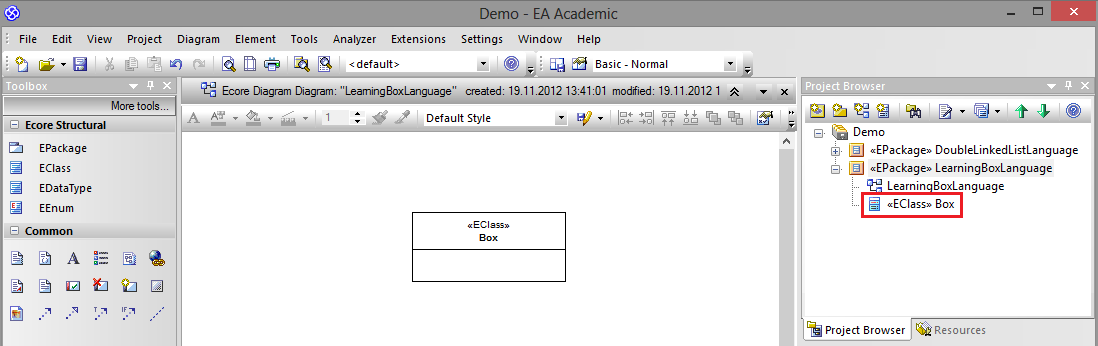
\includegraphics[width=1\textwidth]{ea_afterBoxCreation}
	\caption{State after creating \texttt{Box}}
	\label{ea:eclass_completed}
\end{figure}

\item Now create the \texttt{Partition} and \texttt{Card} EClasses the same way, until your workspace resembles
\Cref{ea:all_eclasses}. These are the main classes of your learning box metamodel.

\vspace{0.5cm}

\item Lets add some attributes! Either right-click on \texttt{Box} to activate the context menu and choose ``Features \&
Properties/Attributes..'' (\Cref{ea:attribute}), or press \texttt{F9} to open the editing dialogue.

\begin{figure}[htbp]
	\centering
  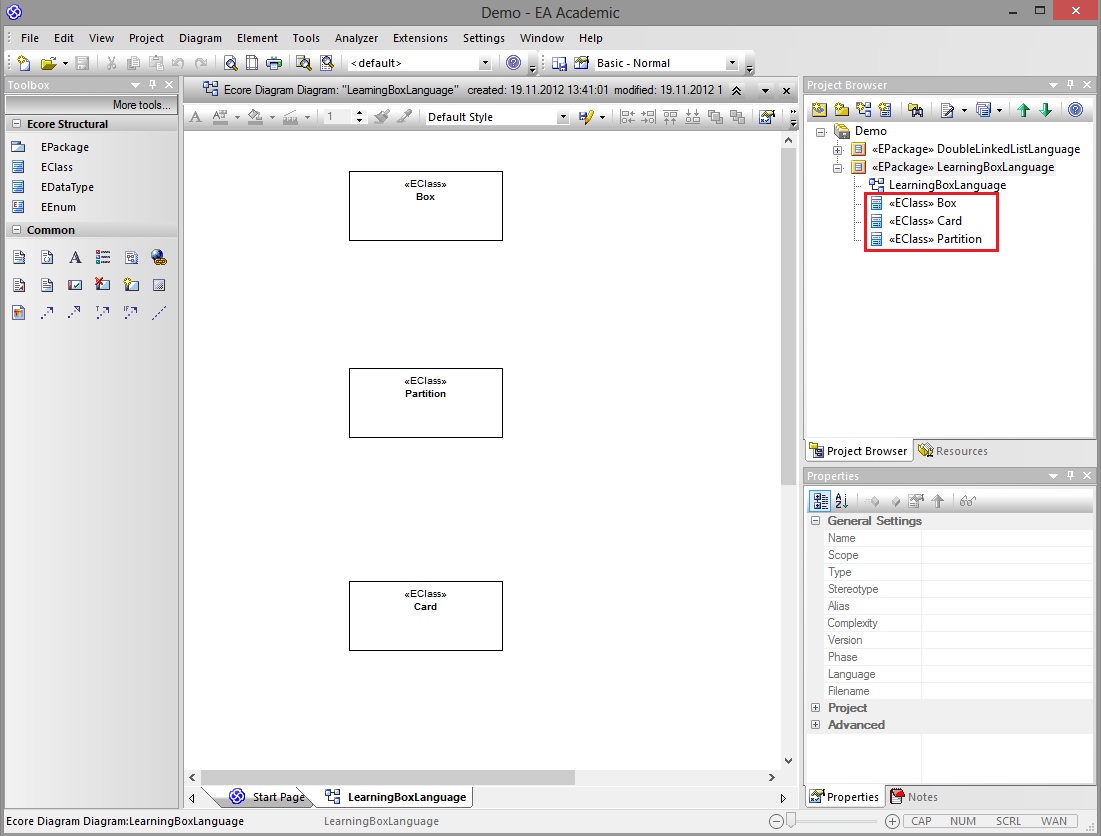
\includegraphics[width=\textwidth]{ea_createPartitionCard}
	\caption{All EClasses for the metamodel}
	\label{ea:all_eclasses}
\end{figure}

\begin{figure}[htbp]
	\centering
  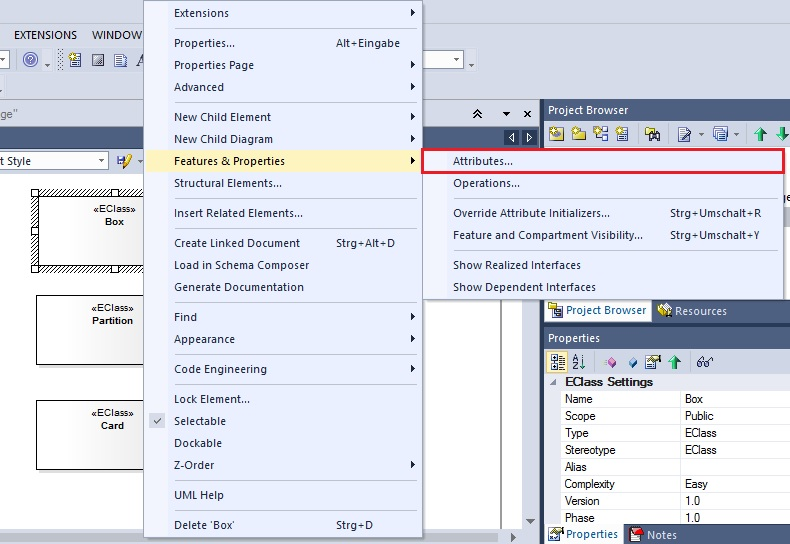
\includegraphics[width=\textwidth]{ea_contextAddAttribute}
	\caption{Context menu for an EClass}
	\label{ea:attribute}
\end{figure}
\FloatBarrier

\item Enter \texttt{name} as the name of the attribute, select \texttt{EString} as its type from the drop-down menu, and press
\texttt{Close} (\Cref{ea:attribute_properties}). New attributes for the same EClass can be added by clicking on \texttt{New Attribute}...\,.

\vspace{1.0cm}

\begin{figure}[htbp]
	\centering
  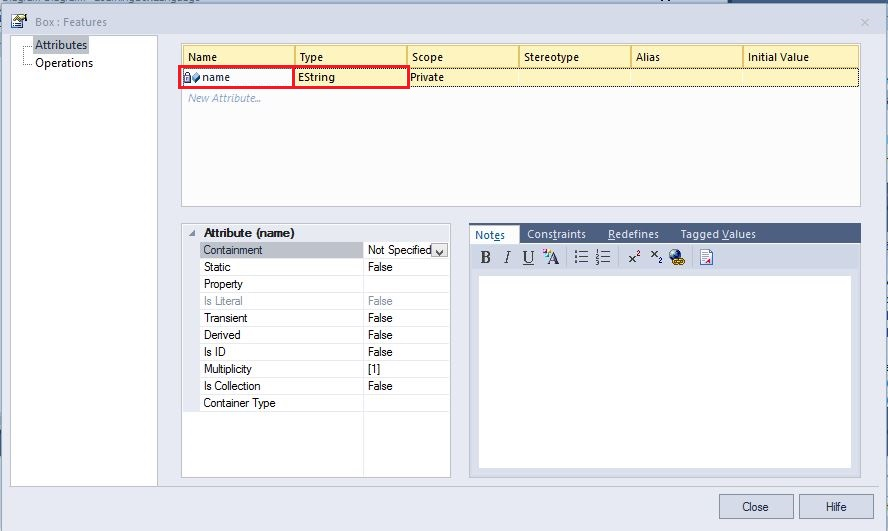
\includegraphics[width=0.9\textwidth]{ea_addAttributesDialogue}
	\caption{Adding attributes to an EClass}
	\label{ea:attribute_properties}
\end{figure}

\vspace{0.5cm}

\item Add the remaining attributes analogously to each EClass until your workspace resembles \Cref{ea:attribute_completed}.

\vspace{0.5cm}

\item Save and export to Eclipse. After refreshing your workspace, your \texttt{.ecore} model can now be expanded as it includes
every class and attribute from your metamodel. So far, so good!

\newpage

\vspace*{3cm}

\begin{figure}[htbp]
	\centering
  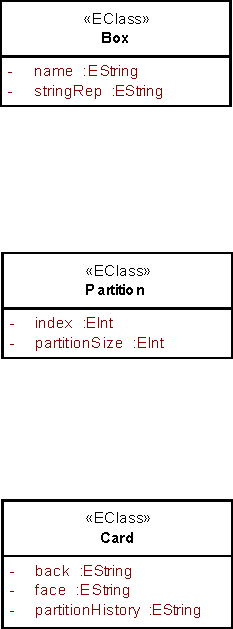
\includegraphics[width=0.40\textwidth]{ea_allAttributes}
	\caption{Main EClasses declared with their attributes}
	\label{ea:attribute_completed}
\end{figure}
\FloatBarrier

\end{stepbystep}

\newpage
\hypertarget{static:classes tex}{}
\subsection{Declaring classes and attributes}
\texHeader

\begin{itemize}

\item[$\blacktriangleright$] Right click your \texttt{LearningBoxLanguage} model and create your first EClass by navigating to ``New/EClass.'' Name it
\texttt{Box}.

\vspace{0.5cm}

\item[$\blacktriangleright$] The class editor should automatically open. Let's add the first two EAttributes of our \texttt{Box}, \texttt{name} and
\texttt{stringRep}. eMoflon offers auto-completion templates to help you with
this task. Go to an empty line and press \texttt{Ctrl + Space}. You'll be
provided with a short list of suggestions (Fig.~\ref{eclipse:typeCompTempl}).
The first four items are related to method control flow, so select \texttt{attribute} near
the bottom to create \texttt{name} of type \texttt{EString}.

\vspace{0.5cm}

\begin{figure}[htbp]
	\centering
  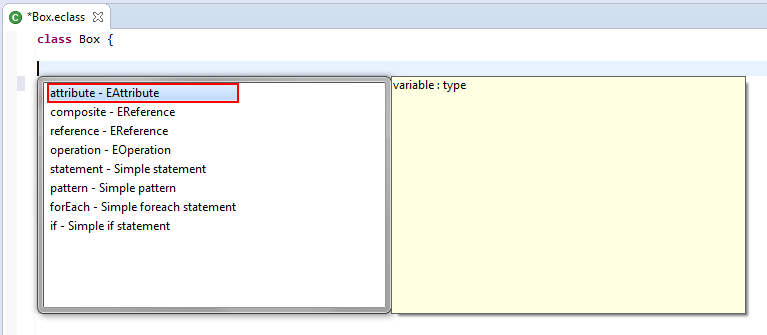
\includegraphics[width=0.6\textwidth]{eclipse_typeCompletionTemplates}
	\caption{eMoflon's auto-completion}
	\label{eclipse:typeCompTempl}
\end{figure} 

\vspace{0.5cm}

\item[$\blacktriangleright$] Auto-completion also supports you by suggesting a list of types. Start to create a second attribute, \texttt{stringRep}, but
stop after typing the \texttt{`:'} operator and press the hotkeys. The pop-up list provides a list of all types currently available
(Fig.~\ref{eclipse:typeCompTypes}) in both your metamodel, and eMoflon's standard metamodels that are included in every new project.

\vspace{0.5cm}

\item[$\blacktriangleright$] Your workspace should now resemble (Fig.~\ref{eclipse:boxDeclaration}).

\newpage

\begin{figure}[htbp]
	\centering
  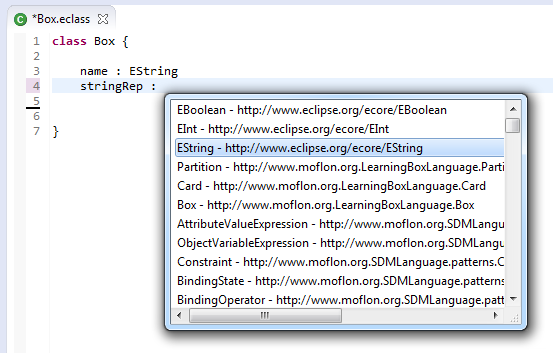
\includegraphics[width=0.6\textwidth]{eclipse_typeCompletionTypes}
	\caption{Type suggestions for \texttt{stringRep}}
	\label{eclipse:typeCompTypes}
\end{figure} 

\vspace{0.5cm}

\begin{figure}[htbp]
	\centering
  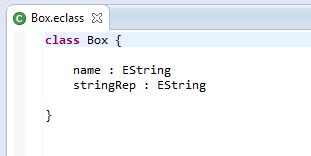
\includegraphics[width=0.5\textwidth]{eclipse_classBoxDeclaration}
	\caption{Newly created \texttt{Box} EClass}
	\label{eclipse:boxDeclaration}
\end{figure} 
\FloatBarrier

\vspace{0.5cm}

\item[$\blacktriangleright$] Now create two empty EClasses in your model, \texttt{Partition} and \texttt{Card}.

\vspace{0.5cm}

\item[$\blacktriangleright$] In \texttt{Partition}, add two \texttt{EInt} attributes, \texttt{index} and \texttt{partitionSize}.

\vspace{0.5cm}

\item[$\blacktriangleright$] In \texttt{Card}, create three \texttt{EString} attributes, \texttt{back}, \texttt{face} , and \texttt{part\-it\-ion\-His\-tory}.

\item[$\blacktriangleright$] If you've done everything correctly, your workspace should now resemble Fig.~\ref{eclipse:workspaceClassAttributes}.

\begin{figure}[htbp]
	\centering
  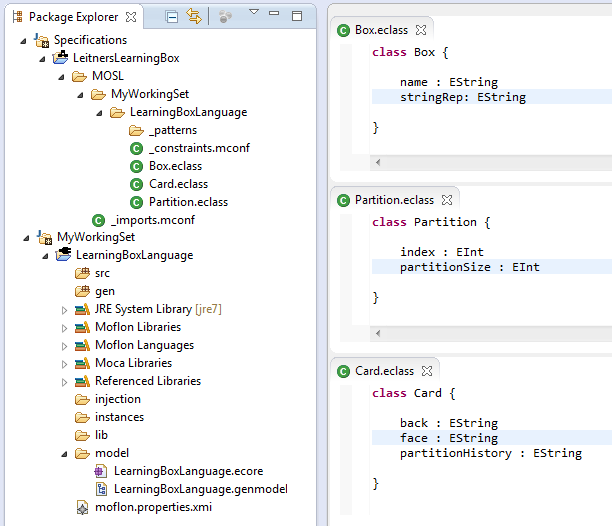
\includegraphics[width=1.0\textwidth]{eclipse_workspaceTexClassAttributes}
	\caption{Declaration of all EClasses and attributes}
	\label{eclipse:workspaceClassAttributes}
\end{figure} 

\vspace{0.5cm}

\item[$\blacktriangleright$] That's it for declaring class attributes! Feel free to build your project again and view the changes in the \texttt{.ecore}
mode, and the generated files in ``gen" and ``src." On a final note, while some languages (such as Java) allow the declaration of several small classes (such as
these three) in the same file, when tooling with eMoflon, we keep them separated. Don't worry -- we'll explain this later in the handbook. As for now, continue
to the next section to start creating references between these EClasses.

\end{itemize}


\newpage
\subsubsection{Creating EReferences in EA}
\visHeader
\hypertarget{static:references vis}{}

\begin{itemize}

\item[$\blacktriangleright$] A fundamental gesture in EA is \emph{Quick Link}. Quick Link is used to create EReferences between elements in a context-sensitive
manner. To use quick link, choose an element and note the little black arrow in its top-right corner (Fig.~\ref{fig:quicklink}).

\begin{figure}[htbp]
	\centering
  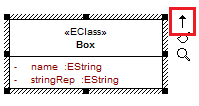
\includegraphics[width=0.4\textwidth]{ea_quickLink}
	\caption{Quick Link is a central gesture in EA}
	\label{fig:quicklink}
\end{figure}
\FloatBarrier

\item[$\blacktriangleright$] Click this black arrow and `pull' to the element you wish to link to. To start, quick-link from \texttt{Box} to \texttt{Partition}.
In the context menu that appears, select ``Create Bidirectional EReference'' (Fig.~\ref{fig:ereference}).

\begin{figure}[htbp]
	\centering
  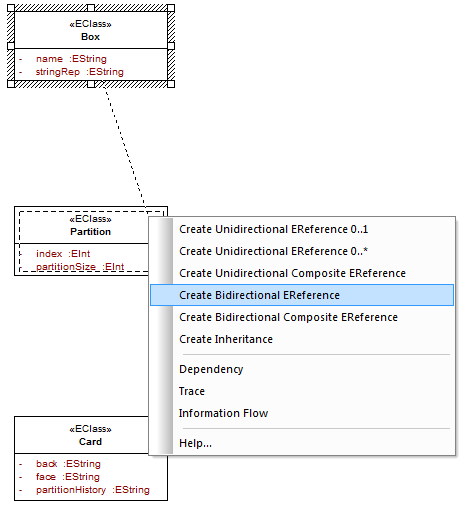
\includegraphics[width=0.6\textwidth]{ea_eReferenceBidirectional}
	\caption{Create an EReference via Quick Link}
	\label{fig:ereference}
\end{figure}
\FloatBarrier

\item[$\blacktriangleright$] Double click the EReference to invoke a dialogue. In this window you can adjust all relevant settings. Feel free to leave the
\texttt{Name} value blank - this property is only used for documentation purposes, and is not relevant for code generation.

\item[$\blacktriangleright$] Within this dialogue, go to ``Source Role,'' and compare the relevant values in Fig.~\ref{fig:role_source} for the \emph{source}
end of the EReference (the \texttt{Box} role). As you can see, the default source is set to the EClass you linked from, while the default target
is the EClass you linked to. In this window, do not forget to confirm and modify the \texttt{Role}, \texttt{Navigability}, \texttt{Multiplicity}, and
\texttt{Aggregation} settings for the source as required. Repeat the process for the \texttt{Target Role} (Fig.~\ref{fig:role_target}).

\vspace{0.5cm}

\begin{figure}[htbp]
	\centering
    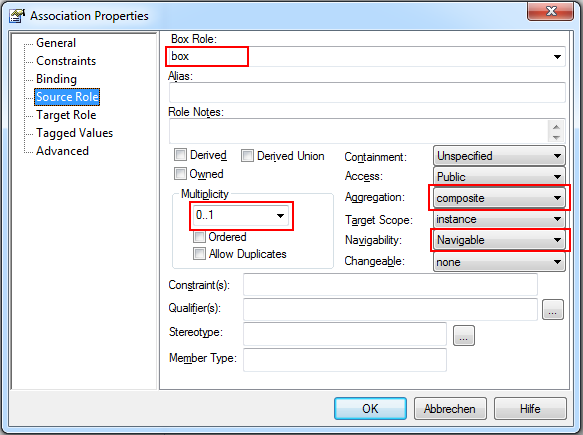
\includegraphics[width=0.9\textwidth]{ea_assocPropsSource}
	\caption{Properties for the source role of an EReference}
	\label{fig:role_source}
\end{figure}

\begin{figure}[htbp]
	\centering
	  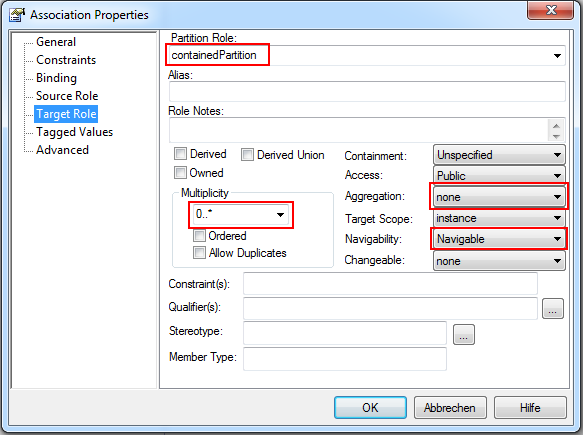
\includegraphics[width=0.9\textwidth]{ea_assocPropsTarget}
	\caption{Properties for the target role of an EReference}
	\label{fig:role_target}
\end{figure}

\end{itemize}

To review these properties, the first value you edited was the role name. The \texttt{Navigation} value should have been automatically set to
\texttt{Na\-vi\-ga\-ble}. Without these two settings, getter and setter methods will not be generated.

Next, you set the \texttt{Multiplicity} value.  In your source role (\texttt{Box}), you have allowed the creation of up to one target (\texttt{Partition})
reference for every connected source (\texttt{box}). This means you could not have a single target connected to two sources (i.e., one partition that belongs to
two boxes). In the target (\texttt{Partition}) role, you have specified that any source (in our case, \texttt{box}) can have any positive-sized number of targets.
Figure~\ref{fig:sketch_roles} sketches this schematically.

\vspace{0.5cm}

\begin{figure}[htbp]
	\centering
    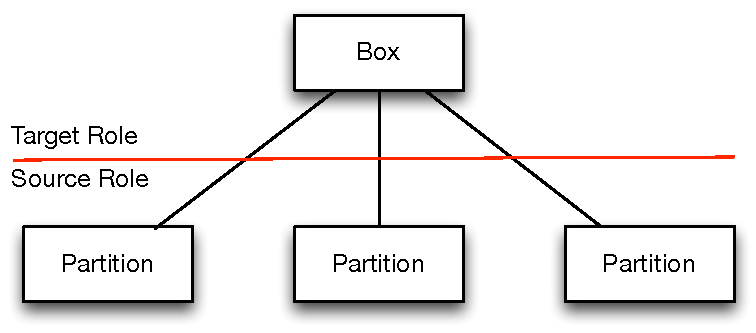
\includegraphics[width=0.6\textwidth]{sketch_multiplicities.pdf}
	\caption{The target and source roles of Leitner's Learning Box}
	\label{fig:sketch_roles}
\end{figure}
\FloatBarrier

Finally, you set the \texttt{Aggregation} value. In this case, \texttt{box} is a container for \texttt{Partition}s, and \texttt{containedPartition} is
consequently not.

\begin{itemize}
\item[$\blacktriangleright$] Take a moment to review how the \texttt{Aggregration} settings extend the \texttt{Multiplicity} rules. If you've done everything
right, your metamodel should now resemble Fig.~\ref{fig:ereference_completed}, with a single \emph{bidirectional EReference} between \texttt{Box} and
\texttt{Partition}.

\vspace{1cm}

\begin{figure}[htbp]
	\centering
  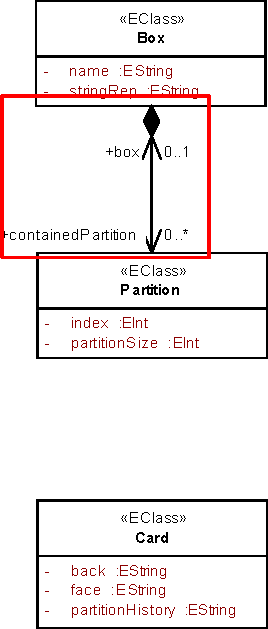
\includegraphics[width=0.35\textwidth]{ea_relationBoxPartition.pdf}
	\caption{\texttt{Box} contains \texttt{Partition}s}
	\label{fig:ereference_completed}
\end{figure}
\FloatBarrier

\item[$\blacktriangleright$] Following the same process, create two unidirectional self-EReferences for \texttt{Partition}, and then a second bidirectional
EReference\footnote{To be precise, \emph{all} EReferences in Ecore are actually unidirectional. A ``bidirectional'' EReference in our metamodel is really two
mapped EReferences that are opposites of each other. We however, believe it is simpler to handle these pairs as single EReferences, and prefer this
concise concrete syntax.} between \texttt{Partition} and \texttt{Card} (Fig.~\ref{fig:ereferences_all}). 

\vspace{1cm}

\begin{figure}[htbp]
	\centering
  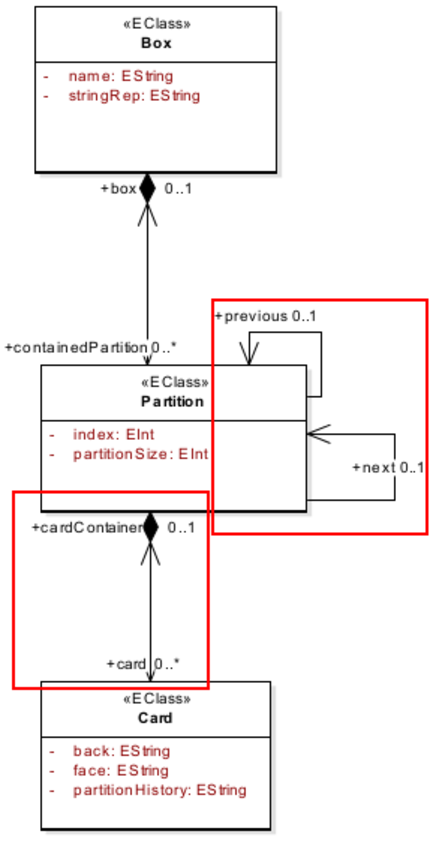
\includegraphics[width=0.7\textwidth]{ea_classAttributes}
	\caption{All relations in our metamodel}
	\label{fig:ereferences_all}
\end{figure}
\FloatBarrier

\vspace{1cm}

\item[$\blacktriangleright$] You'll notice that the connection between \texttt{Card} and \texttt{Partition} is similar to that between \texttt{Partition} and
\texttt{Box}. This makes sense as a partition should be able to hold an unlimited amount of cards, but a card can only belong to one partition at a time.

\vspace{1cm}

\item[$\blacktriangleright$] Export your diagram to Eclipse and refresh your workspace. Your Ecore file should now resemble Fig~\ref{fig:model_allClasses}.

\vspace{1cm}

\begin{figure}[htbp]
	\centering
  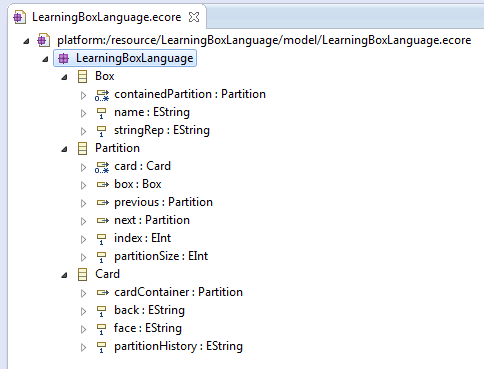
\includegraphics[width=0.7\textwidth]{eclipse_modelDeclaredClasses}
	\caption{Refreshed Ecore file with all EReferences}
	\label{fig:model_allClasses}
\end{figure}

\vspace{1cm}

\item[$\blacktriangleright$] All the required attributes and references for your learning box have now been set up. We encourage you to see how these are
declared in the textual syntax, starting on the immediate next page. In particular, check out Fig.~\ref{fig:allReferences}, where each EClass is fully
declared, and Fig.~\ref{fig:bothConstraints}, where bidirectionality is explicitly specified as a constraint.

\jumpSingle{static:methods vis}

\end{itemize}

\newpage
\subsubsection{Connecting your classes with MOSL}
\texHeader
\hypertarget{static:references tex}{}

In MOSL, the declaration of a reference is simple; the syntax is made up of four parts:  \small{\texttt{[Aggregation Type][Navigation
Name](Multiplicity):[Role]}}. A simple reference is defined with an arrow operator, while a contained reference is a sideways diamond and arrow combination.

% Edit me
To avoid redundancies in your code, it's important to know that both types automatically update the other role involved in the reference, which means you only
have to declare a direction once.


\begin{itemize}

\item[$\blacktriangleright$] Open \texttt{Box} class in the editor and add a \emph{container reference} named \texttt{containedPartition} with a multiplicity of zero
to infinite, of type \texttt{Partition} (Fig.~\ref{fig:cpartitionReference}). This means {\bf THAT}.

\begin{figure}[htbp]
	\centering
  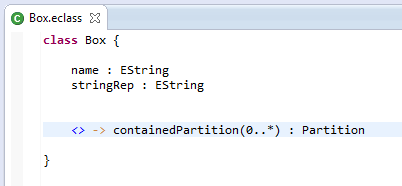
\includegraphics[width=0.6\textwidth]{eclass_box}
	\caption{Creating a \emph{contained reference} in \texttt{Box}}
	\label{fig:cpartitionReference}
\end{figure} 

\item[$\blacktriangleright$] Now add a \emph{simple reference} to \texttt{Partition}. Name it \texttt{box}, and allow it to hold up to one \texttt{Box}
(Fig.~\ref{fig:boxReference}). This means {\bf THAT}.

\begin{figure}[htbp]
	\centering
  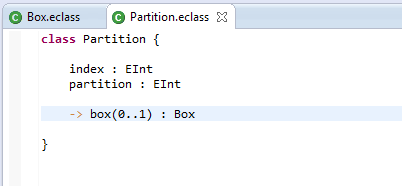
\includegraphics[width=0.6\textwidth]{eclass_partition}
	\caption{Creating a \emph{simple reference} in \texttt{Partition}}
	\label{fig:boxReference}
\end{figure} 

\item[$\blacktriangleright$] Congratulations, you have just built your first pair of EReferences. This pair is also known as a \emph{Bidirectional
EReference}! To see how this is depicted visually, check out Fig.~\ref{fig:ereference_completed} in the previous subsection.

\newpage

\item[$\blacktriangleright$] Now, lets create another EReference pair, or bidirectional EReference, between \texttt{Partition} and \texttt{Card}. If you think
about it, it's really not all that different than the relation between \texttt{Box} and \texttt{Partition}. In fact, it's not different at all! A
\texttt{Partition} should be able to hold an unlimited amount of \texttt{Card}s, but a \texttt{Card} should only be allowed to belong to zero or one
\texttt{Partition}s. Name the two new relations \texttt{containedPartition}, and \texttt{box}.

\item[$\blacktriangleright$] Your classes should now closely resemble Fig.~\ref{fig:almostAllReferences}.

\begin{figure}[htbp]
	\centering
  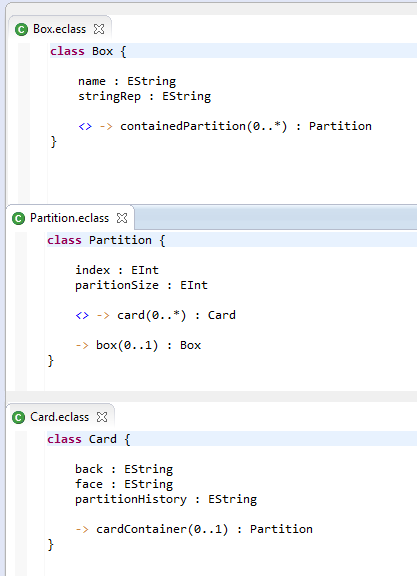
\includegraphics[width=0.65\textwidth]{eclipse_workspaceReferences}
	\caption{The Completed Bidirectional EReferences}
	\label{fig:almostAllReferences}
\end{figure} 

\item[$\blacktriangleright$] The next step is to set up two relations between \texttt{Partition} and itself, so it can shift between the previous and next
partition in the box. Create two new simple references, named \texttt{previous}, and \texttt{next}. Allow them to have a maximum of 1 link each.

\item[$\blacktriangleright$] All of our references are now set up! If you have done everything correctly, your classes should now resemble Fig.~\ref{fig:allReferences}.
To see how all of this is depicted visually, check out Fig.~\ref{fig:ereferences_all} in \hyperlink{sec:static vis}{section 2.1}.

\begin{figure}[htbp]
	\centering
  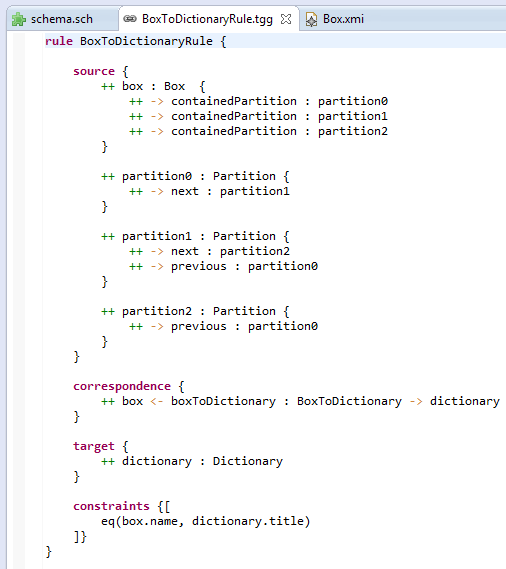
\includegraphics[width=0.6\textwidth]{eclipse_allReferences}
	\caption{All references in Leitner's Learning Box}
	\label{fig:allReferences}
\end{figure} 

\fancyfoot[R]{$\triangleright$ \hyperlink{static:methods tex}{Next}}
\end{itemize}


\newpage
\subsection{Method Signatures}
\genHeader
\hypertarget{static:methods vis}{}

To finish defining our types, lets define the \emph{signatures}\define{Operation Signature} of some operations that they'll eventually support.

\begin{stepbystep}

\item  Select \texttt{Partition} and either right-click to invoke the context-menu (\Cref{ea:add_operation})  and choose ``Features \&
Properties/Operations..'' or simply press \texttt{F10}.

\begin{figure}[htbp]
	\centering
  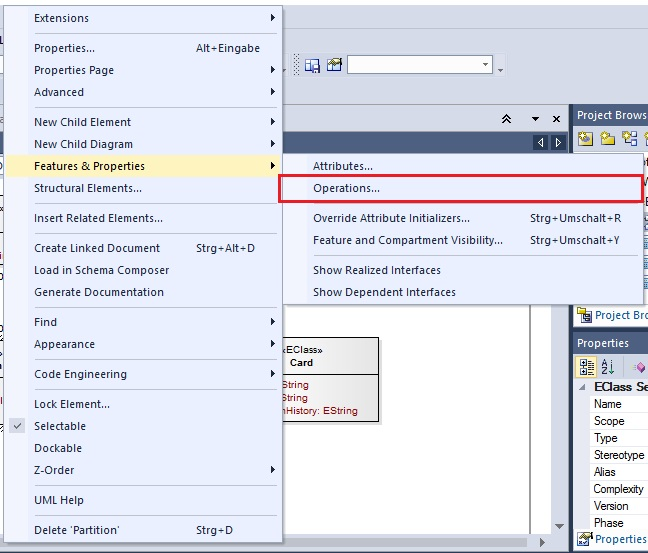
\includegraphics[width=0.8\textwidth]{../../org.moflon.doc.handbook.02_leitnersLearningBox/2_staticSemantics/4_creatingMethods/cmVisImages/ea_contextAddOperation}
	\caption{Add an operation}
	\label{ea:add_operation}
\end{figure}
\FloatBarrier

\item  In the dialogue that pops-up (\Cref{ea:operation_properties}), enter \texttt{empty} as the \texttt{Name} of the operation and \texttt{void} as the \texttt{Return Type}.

\vspace{0.5cm}

\item  In the same dialogue, click on \texttt{New Operation...} to add a second operation, \texttt{removeCard}, and edit the values as seen in 
\Cref{ea:operation_parameters}. Notice that the \texttt{Return Type} can be chosen by either the drop-down menu, or via direct typing. For types you've established in
the metamodel (e.g. \texttt{Card}) you have to use `\texttt{Select Type...}' from the drop-down menu.
\vspace{-.3cm}
\begin{quote}
{ \small
$\textbf{Very important:}$ Non-primitive types \emph{must} be chosen via `\texttt{Select Type...}' in the drop-down menu. It allows you to browse for the corresponding elements in
your project. Simply typing them won't work!
}
\end{quote}

\begin{figure}[htbp]
	\centering
  	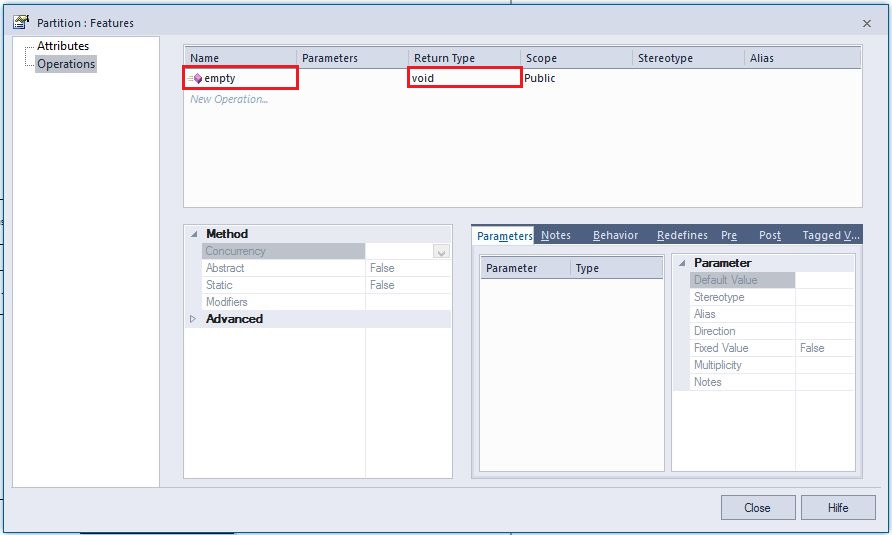
\includegraphics[width=\textwidth]{../../org.moflon.doc.handbook.02_leitnersLearningBox/2_staticSemantics/4_creatingMethods/cmVisImages/ea_operationEmpty}
	\caption{EClass properties editor}
	\label{ea:operation_properties}
\end{figure}


\item  Parameters can be added by selecting \texttt{Parameters} and
completing the dialouge (\Cref{ea:operation_parameters}). Please remember that you must also use either the drop-down menu, or direct typing to select the type or else validation
will fail.

\item  Repeat this process for the \texttt{check} operation (with the two parameters \texttt{card:Card, guess:EString}) that returns an \texttt{EBoolean}. 

\item  If you've done everything right, your dialogue should now contain three methods - \texttt{check}, \texttt{empty}, and
\texttt{removeCard} - each with the corresponding parameters and return types in \Cref{ea:operation_partition}.


\item  Add all operations analogously for \texttt{Box} and \texttt{Card} until your metamodel closely resembles
\Cref{ea:metamodel_complete}.\footnote{Please note that names of parameters may not be displayed by default in EA}

\item  To finish, export the metamodel for code generation in Eclipse, and examine the model once again. Each signature should have
appeared in their respective EClass.

\newpage

\vspace*{1cm}

\begin{figure}[htbp]
	\centering
  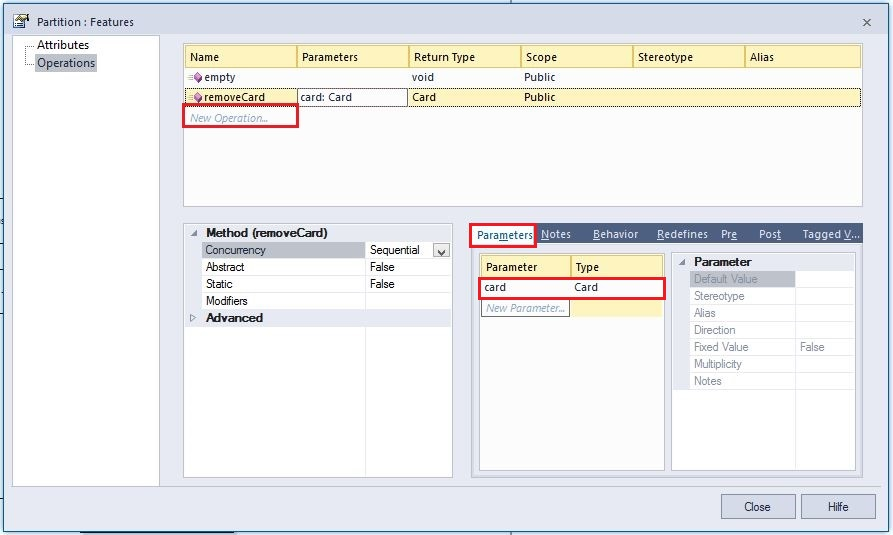
\includegraphics[width=\textwidth]{../../org.moflon.doc.handbook.02_leitnersLearningBox/2_staticSemantics/4_creatingMethods/cmVisImages/ea_operationRemoveCard}
	\caption{Parameters and return type}
	\label{ea:operation_parameters}
\end{figure}

\vspace{1cm}

\begin{figure}[h!]
	\centering
  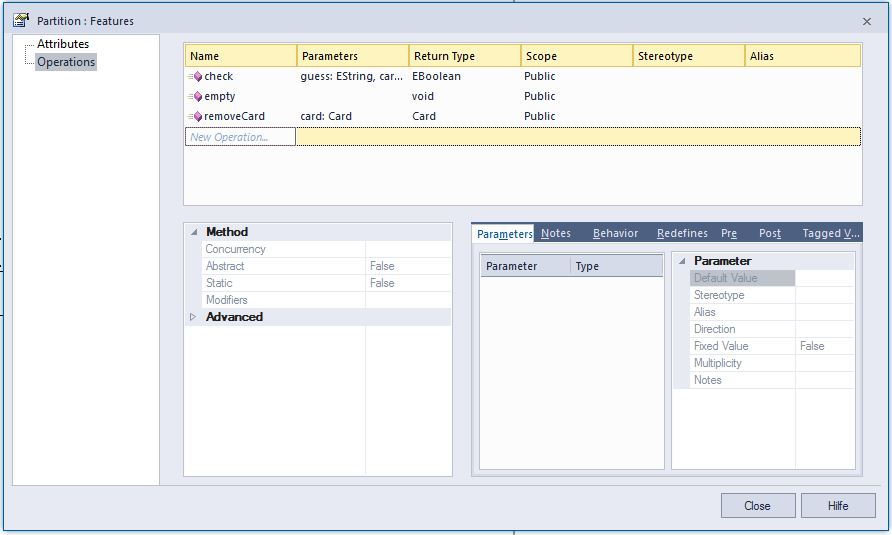
\includegraphics[width=\textwidth]{../../org.moflon.doc.handbook.02_leitnersLearningBox/2_staticSemantics/4_creatingMethods/cmVisImages/ea_operationCheck}
	\caption{All operations in \texttt{Partition}}
	\label{ea:operation_partition}
\end{figure}

\newpage


\begin{figure}[htbp]
	\centering
  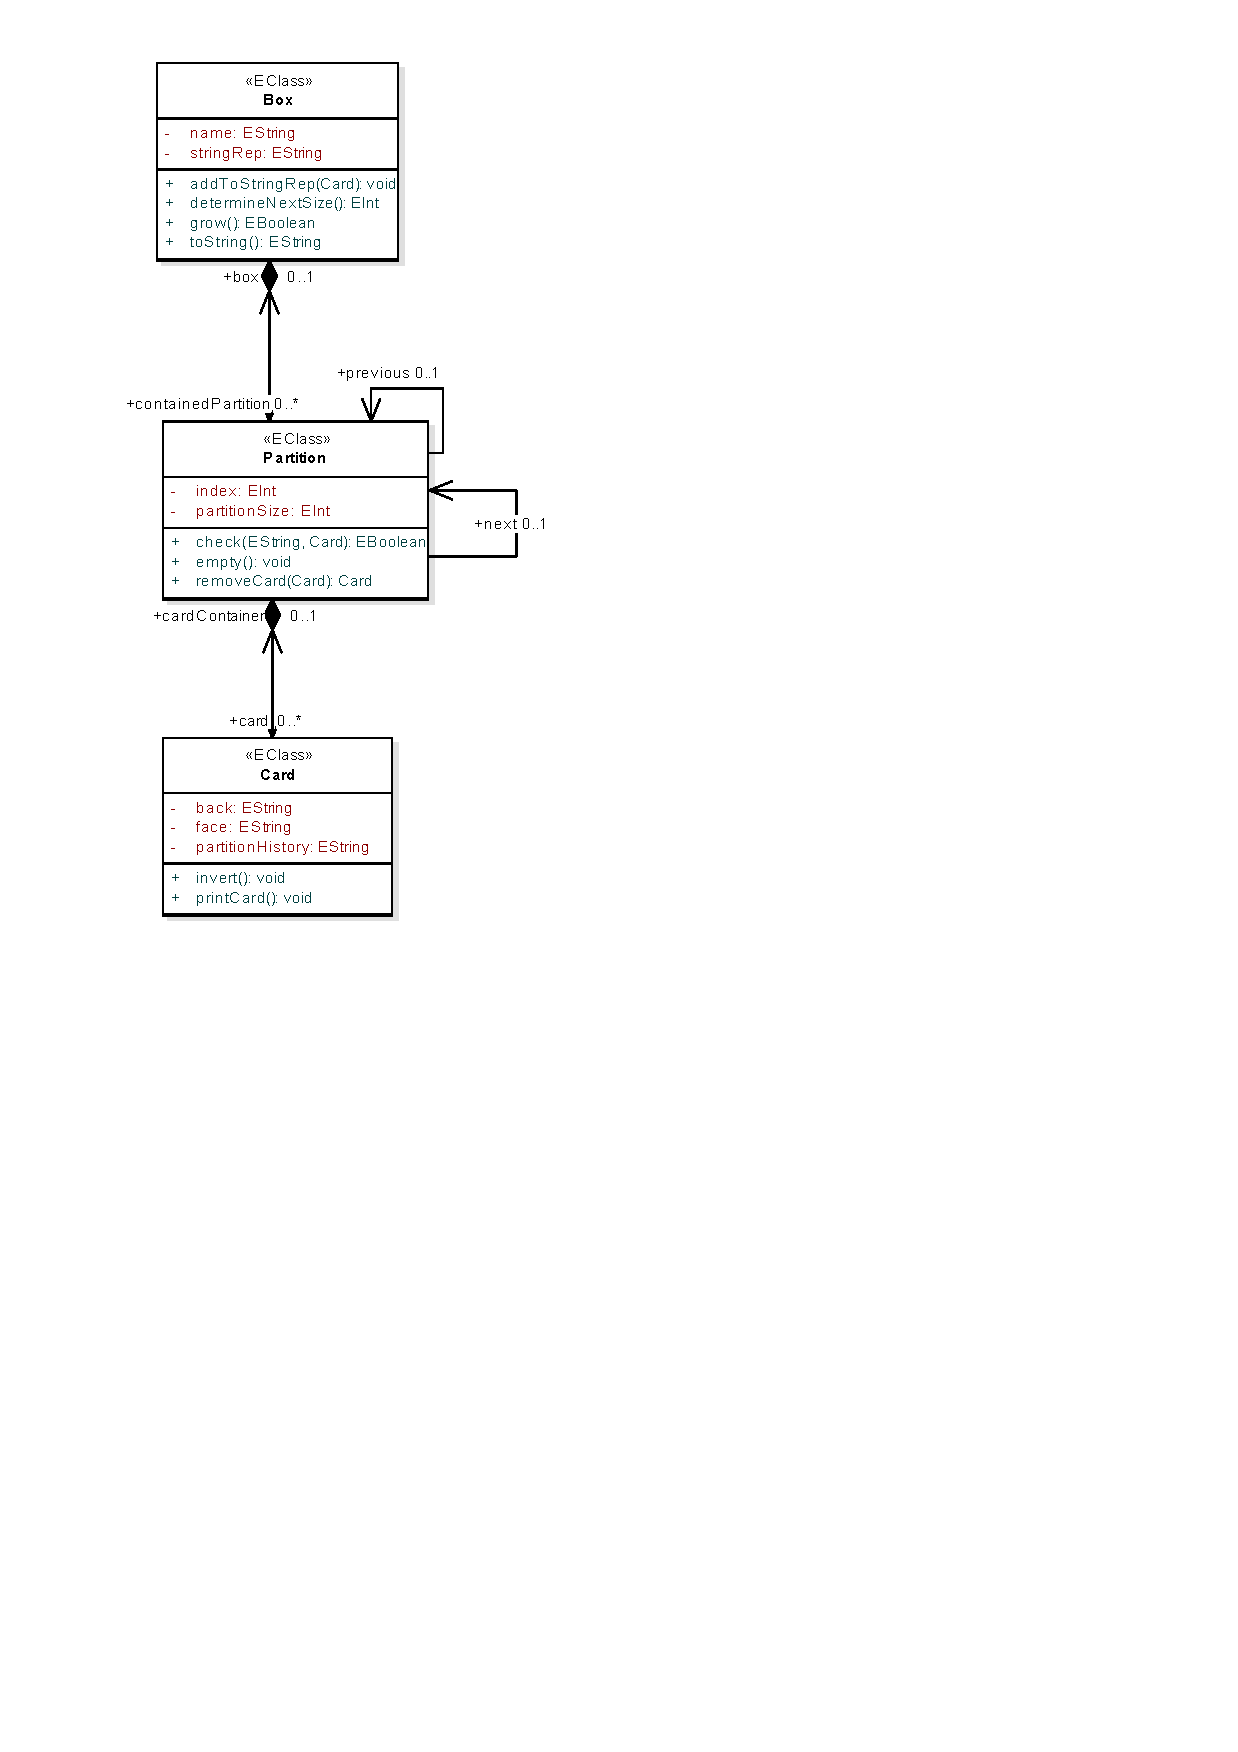
\includegraphics[width=0.6\textwidth]{../../org.moflon.doc.handbook.02_leitnersLearningBox/2_staticSemantics/4_creatingMethods/cmVisImages/ea_metamodelComplete}
\caption[Complete metamodel for our learning box.]{Complete metamodel for our learning box}
	\label{ea:metamodel_complete}
\end{figure}
\FloatBarrier

\end{stepbystep}

\newpage
\subsection{Method Signatures}
\texHeader
\hypertarget{static:methods tex}{}

\begin{itemize}

\item[$\blacktriangleright$] We're nearing the end of our model creation! One of the last things we need to do is to make the model \emph{do} something. After
all, a model that only stores attributes and references is a bit boring, right?

\item[$\blacktriangleright$] Let's set up the operations we want each EClass to do by declaring their \emph{signatures} which follow the syntax below:
\syntax{name `(' argument* `)' `:' return\_type \\
\\
With:\\
name, arguments, return\_type := STRING}

\item[$\blacktriangleright$] Starting with the \texttt{Partition} EClass, we want a partition to be able to do three things: compare the answer on a
\texttt{Card} with a guess and return a true/false response, remove a specific card from the partition, or empty itself of all cards.

\item[$\blacktriangleright$] Start with the \texttt{empty} method. It won't need any parameters, and it doesn't return anything. Declare this via:
\syntax{empty() : void}

\item[$\blacktriangleright$] Create two more functions for \texttt{Partition} the same way. We'll need a \texttt{removeCard} method that accepts and returns a
\texttt{Card}, as well as a EBoolean \texttt{check} method that accepts a \texttt{Card} and an \texttt{EString} guess. 

\item[$\blacktriangleright$] Your \texttt{Partition} EClass should now resemble Fig.~\ref{eclipse:partitionMethods}.

\vspace{0.5cm}

\begin{figure}[htbp]
	\centering
  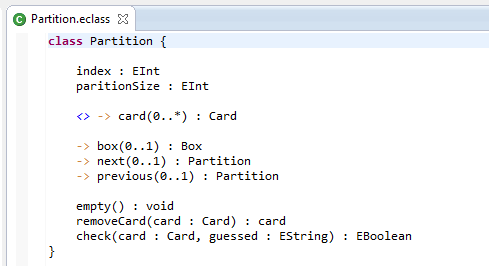
\includegraphics[width=0.6\textwidth]{eclipse_partitionMethods}
	\caption{The completed \texttt{Partition} EClass}
	\label{eclipse:partitionMethods}
\end{figure}

\vspace{0.5cm}

\item[$\blacktriangleright$] What needs to be done in the \texttt{Card} EClass? Well, in order to check the card, we'll need to be able to look at the flip
side. We'll also need to print whatever is on the current side. Create two paramater-less \texttt{void} functions, \texttt{invert} and \texttt{printCard}. 

\item[$\blacktriangleright$] Finally, what do we want to do with \texttt{Box}? In summary, we want a \texttt{Box} to:

\begin{description}
  \item[\texttt{determineNextSize():EInt}] Calculate how large a new partition in the box should be
  \item[\texttt{grow():EBoolean}] Increase the box by adding a new partition
  \item[\texttt{toString():EString}] Produce a string representation of the box with all its contents
  \item[\texttt{addToStringRep(card:Card):void}] Update the current string representation to include \texttt{card}
\end{description}

\item[$\blacktriangleright$] Implement the above signatures, and your entire workspace should now resemble Fig.~\ref{eclipse:workspaceMethods}.

\item[$\blacktriangleright$] Congratulations! You have now created a metamodel for our Learning Box using eMoflon's textual syntax! To see how
this looks in the visual syntax, check out Fig.~\ref{ea:metamodel_complete} from the previous section. As a final step, make sure you build the project and
wait for the package explorer to refresh. 

\newpage

\jumpSingle{validation tex}

\begin{figure}[htbp]
	\centering
  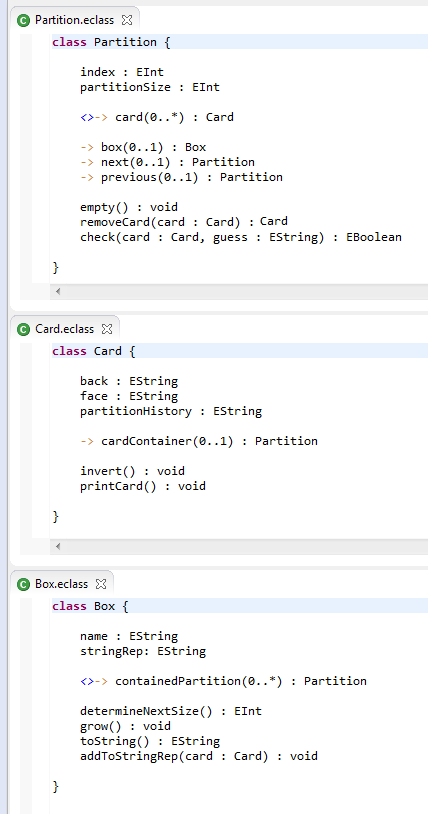
\includegraphics[width=0.7\textwidth]{eclipse_classesFullyDeclared}
	\caption{Completed method signatures}
	\label{eclipse:workspaceMethods}
\end{figure}
\FloatBarrier

\end{itemize}

\newpage 
\genHeader
\subsection{Reviewing your metamodel}
\hypertarget{static review}{}

Congratulations on completing the abstract syntax of your metamodel! Before moving on, lets take a step back and review. We have modelled a \texttt{Box} that
can contain an arbitrary amount of \texttt{Partition}s. A \texttt{Partition} in the \texttt{Box} has a \texttt{next} and \texttt{previous} \texttt{Partition}
that can or not be set. Finally, \texttt{Partition}s contain \texttt{Card}s.

A \texttt{Box} has a \texttt{name}, and can be extended by calling \texttt{grow}. A \texttt{Box} can print out its contents via the \texttt{toString} method.

The main method of the learning box is \texttt{Partition::check}, which takes a \texttt{Card} and the user's \texttt{EString} guess, and returns a \texttt{true}
or \texttt{false} value.

A \texttt{Partition} can also \texttt{remove} a specific \texttt{Card}, or empty itself of all  existing \texttt{Cards}. Last but not least, a
\texttt{Partition} has a \texttt{partitionSize} to indicate how many cards it currently has. Too many cards in the first partition could indicate that not
enough time has been dedicated to learning the terms. Too many near the end could show that the vocabulary set is too easy, and probably mastered.

A \texttt{Card} contains the actual content to be learned as a question on the card's \texttt{face} and the answer on the card's \texttt{back}. A \texttt{Card}s
also maintain \texttt{partition\-History}, which can be used to keep track of how often a \texttt{Card} has been answered incorrectly.
This may indicate how difficult the \texttt{Card} is for a specific user, and remind them to spend more time on that set. When learning a language, it makes
sense to be able to swap the target and source language and this is supported by \texttt{Card} via \texttt{invert} (turns the card around).

On a final note, we encourage you to review how the program was constructed in the syntax \emph{opposite} to the one you just used. Compare the differences
between modelling classes and references in diagrams using a separate program, then exporting to Eclipse to build, versus modelling entirely within the Eclipse
IDE with various commands. Which do you find easier to work with?

If you have had problems with this section, and, despite firmly believing everything is correct, things still don't work, feel free to contact us at 
\href{mailto:contact@moflon.org}{contact@moflon.org}.

\fancyfoot[R]{ $\triangleright$ \hyperlink{validation vis}{Next [visual]\hspace{0.2cm}} \\ $\triangleright$ \hyperlink{validation tex}{Next [textual]}}
 


\newpage
\genHeader

\section{Creating instances}
\hypertarget{sec:creatingInstance common}{}

Before diving into modelling dynamic behaviour in Part III, let's have a brief look at how to create a concrete \emph{instance} of your abstract syntax in
Eclipse.

\vspace{0.5cm}

In the following section, we use \emph{metamodel} and \emph{instance model} to differentiate between models that represent the abstract syntax and static
semantics of a domain specific language (metamodel), and those that are expressed \emph{in} such a language (instance models of the metamodel).

\begin{itemize}

\item[$\blacktriangleright$] To create an instance model, navigate to the generated \texttt{model} folder in your \texttt{LearningBoxLanguage} project.
Double-click the \texttt{LearningBoxLa\-nguage.ecore} model to invoke  the \emph{Ecore model editor}. The Eclipse Modeling Framework (EMF) provides a generic
tree-model editor which allows us to create and edit an arbitrary instance of any metamodel specified with eMoflon. Expand this tree to review all the classes,
attributes, and signatures you just created.

\vspace{0.5cm}

\item[$\blacktriangleright$] To create a concrete instance of the metamodel, you must select a class that will become the root element of the new instance.
For our example, right-click \texttt{Box}, and navigate to ``Create Dynamic Instance'' from the context menu, as depicted in Fig.~\ref{fig:context_menu}.

\begin{figure}[htbp]
	\centering
  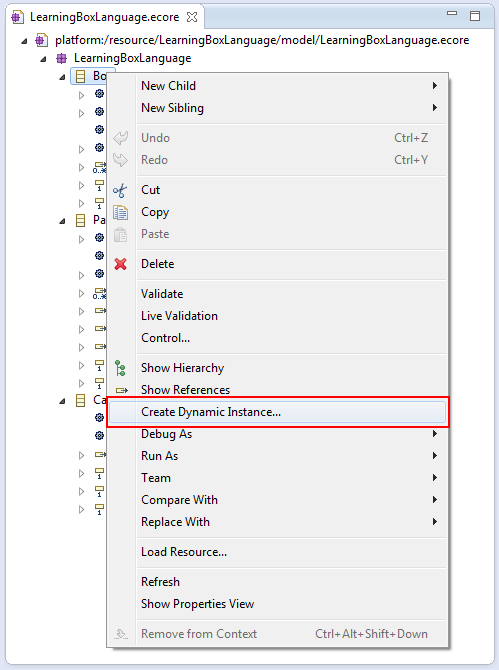
\includegraphics[width=0.6\textwidth]{eclipse_createDynamicInstance}
	\caption{Context menu of an EClass in the Ecore editor}
	\label{fig:context_menu}
\end{figure}

\vspace{0.5cm}

\item[$\blacktriangleright$] A dialogue should appear asking where the instance model file should be persisted. Save your instances according to convention in a
folder named ``instances,'' which is automatically created in every new repository project. Last but not least, enter `Box' as the name of the instance model
(Fig.~\ref{fig:store_dynamic_instance}).

\vspace{0.5cm}

\begin{figure}[htbp]
	\centering
  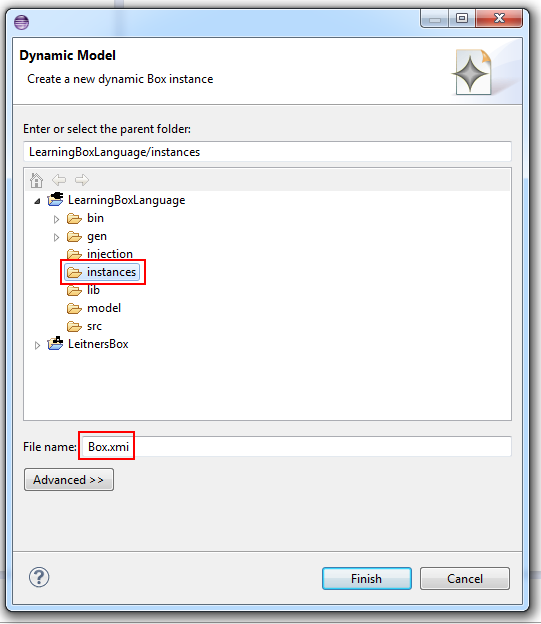
\includegraphics[width=0.6\textwidth]{eclipse_nameDynamicInstance}
	\caption{Dialogue for creating a dynamic model instance}
	\label{fig:store_dynamic_instance}
\end{figure}

\item[$\blacktriangleright$] Press \texttt{Finish}, and the generic model editor should open for your new instance model. This editor works just like the
previous Ecore model editor except it's ``generic,'' meaning it allows you to create and edit an instance of \emph{any} metamodel, not only those using Ecore.

\clearpage

\item[$\blacktriangleright$] You can populate any element of your instance by adding new children or siblings via a right-click of an element to invoke the
context-menu depicted in Fig.~\ref{fig:create_instance}. Note that EMF supports you by respecting your metamodel, and reducing the choice of available elements
to valid types only.\footnote{This depends on the current context. Try it out!}

\begin{figure}[htbp]
	\centering
  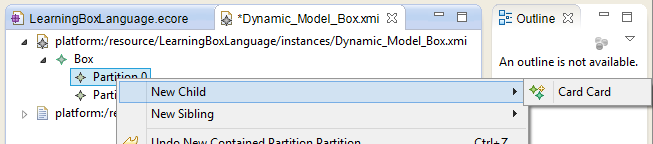
\includegraphics[width=0.8\textwidth]{adjustModel}
	\caption{Context menu for creating model elements}
	\label{fig:create_instance}
\end{figure}

\item[$\blacktriangleright$] Your model as an \texttt{.xmi} file by pressing \texttt{Ctrl+S}. When you close it, the model can be reloaded via a simple
double-click to invoke the generic model editor.

\item[$\blacktriangleright$] Let's try building a vocabulary set. Fill your box with two partitions, each containing three cards.

\item[$\blacktriangleright$] Double click on one of the partitions to bring up the ``Properties'' tab in the window below the editor
(Fig.~\ref{fig:properties_partition}). Here you'll see the attributes you defined earlier in the classes. Pick a number - any one you like - and update the
\texttt{Partition} value. As soon as you hit \texttt{Enter}, you'll see that the change in name has been reflected in the tree. Give the second partition a
unique EInt value as well.

\item[$\blacktriangleright$] Now you need to set the \texttt{Next} and \texttt{Previous} partition values that will make it possible to move cards through the
box. Set every \texttt{Previous} value to the very first partition in your box, then each \texttt{Next} value to the next partition. For the last partition, set
the \texttt{Next} value to itself. 

\item[$\blacktriangleright$] In the same fashion, double click on each \texttt{Card} you created and modify their values. In particular, modify the
\texttt{Back} attribute. Change it to `Null' This is the value you'll see from the partition. You'll be experimenting with the \texttt{Face} attribute shortly,
so provide a `Zero' value for that as well.

\item[$\blacktriangleright$] Fill in the rest the cards with similar vocabulary-style words that you can quiz yourself on. You now have a unique, customized
learning box! Save your model, and ensure no errors exist before proceeding with the final sections of this handbook.

\newpage

\vspace*{4cm}

\begin{figure}[htbp]
	\centering
  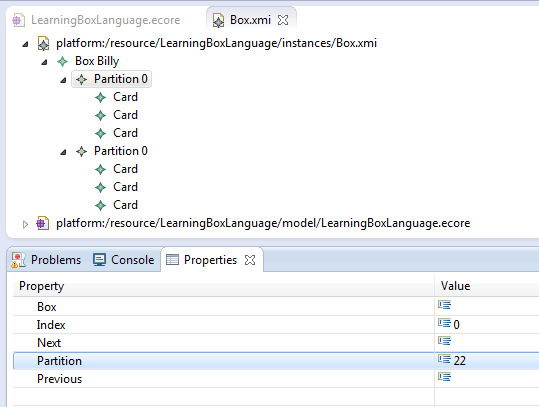
\includegraphics[width=0.8\textwidth]{eclipse_propertiesTab}
	\caption{Change the \texttt{Index} value in the partition's property tab}
	\label{fig:properties_partition}
\end{figure}

% \fancyfoot[R]{ $\triangleright$ \hyperlink{sec:Graph View}{Next}}

\end{itemize}


\newpage
\section{eMoflon's Graph Viewer}
\genHeader

From ecore, drag and drop\ldots may have to edit/open up the window again. Can right click the ``eMoflon'' tab, and press ``Reset'' to reload any windows you
may have accidentally closed. ALternatively, you can go to ``Window/Show View/Other\ldots'' and then to ``Other/Graph View.''


\newpage
\section{Introduction to injections}
\genHeader

This short introduction will show you how to implement small methods by adding handwritten code to classes generated from your model. Injections are inspired by
partial classes in C\#, and are our preferred way of providing a clean separation between generated and handwritten code. 

Let's implement the \texttt{removeCard} method, declared in the \texttt{Partition} EClass. In order to `remove' a card from a partition, all one needs to do is
disable the link between them. Don't forget that (according to the signature) not only does \texttt{removeCard} have to pass in a \texttt{Card}, it must return
one as well.

\begin{itemize}

\item[$\blacktriangleright$] From your working set, open ``gen/LearningBoxLanguage.impl/Part\-it\-ionImpl.java'' and enter the following code in the
\texttt{removeCard} declaration, starting at approximately line 347. Do not remove the first comment, which is necessary to indicate that this code is written
by the user and needs to be extracted automatically as an injection. Please also do not copy and paste the following code -- the copying process will most
likely add invisible characters that eMoflon is unable to handle.

\vspace{0.5cm}

\begin{figure}[htbp]
        \centering
        \begin{lstlisting}[language=Java, keywordstyle={\bfseries\color{purple}}, backgroundcolor=\color{white}]
    public Card removeCard(Card toBeRemovedCard) {
		// [user code injected with eMoflon]
		if(toBeRemovedCard != null){
			toBeRemovedCard.setCardContainer(null);
		}
		return toBeRemovedCard;
	}
        \end{lstlisting}
        \caption{Implementation of \texttt{removeCard}}
        \label{code:addToStringRep_impl}
\end{figure}

\vspace{0.5cm}

\item[$\blacktriangleright$] Save the file, then right-click either on the file in the package explorer, or in the editor window, and choose ``eMoflon/
Create/Update Injection for class'' (Alt+Shift+E,I) from the context menu (Fig.~\ref{eclipse:injection_create_injection}).

\begin{figure}[htbp]
    \centering
    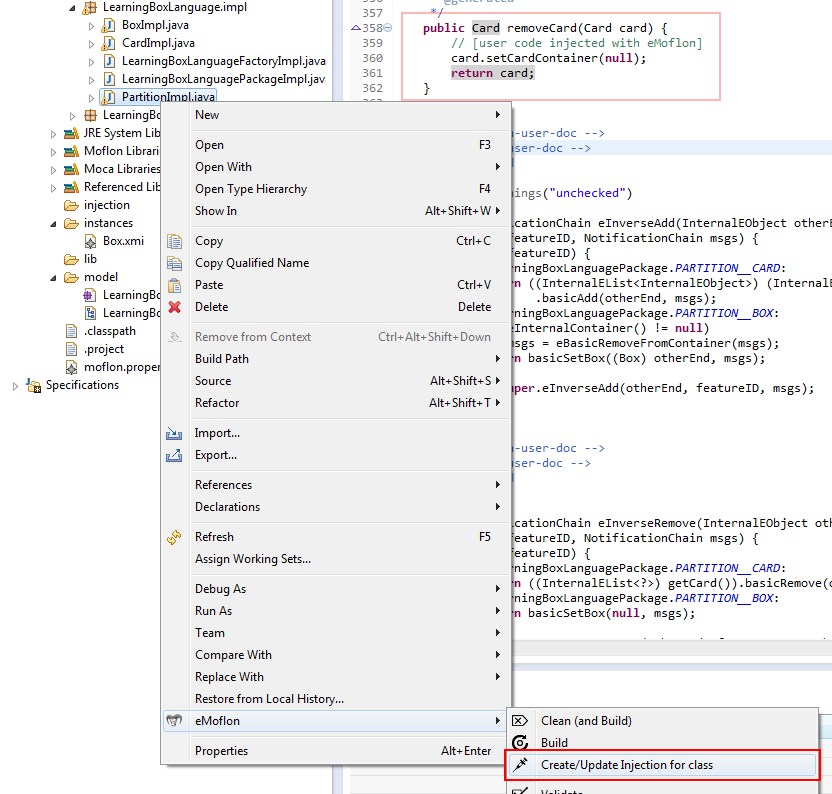
\includegraphics[width=\textwidth]{eclipse_createInjection}
    \caption{Create a new injection}
    \label{eclipse:injection_create_injection}
\end{figure}

\item[$\blacktriangleright$] This will create a new file in the ``injection'' folder of your project with the same package and name stucture as the Java class,
but with a new \texttt{.inject} extension (Fig.~\ref{eclipse:injection_folder}).

\begin{figure}[htbp]
    \centering
    \includegraphics[width=0.5\textwidth]{eclipse_injectionFolder}
    \caption{Partition injection file}
    \label{eclipse:injection_folder}
\end{figure}

\item[$\blacktriangleright$] Double click to open and view this file. It contains the definition of a \textit{partial class}
(Fig.~\ref{eclipse:injection_partialClassPartition}).

\begin{figure}[htbp]
    \centering
    \includegraphics[width=0.8\textwidth]{eclipse_partialClassPartition}
    \caption{Generated injection file for \texttt{PartitionImpl.java}}
    \label{eclipse:injection_partialClassPartition}
\end{figure}

\clearpage

\item[$\blacktriangleright$] As a final step, build your metamodel to check that the code is generated and injected properly.

\item[$\blacktriangleright$] By the way, eMoflon allows you to switch quickly between a Java class and its injection file.
When inside ``PartitionImpl.java", open the context menu and select ``eMoflon/Class \verb|<->| Injection" (Alt+Shift+E,W).
This brings you to ``PartitionImpl.java".

Repeat this command and you are back in ``PartitionImpl.inject``.


\item[$\blacktriangleright$] That's it! While injecting handwritten code is a remarkably simple process, it is pretty boring and low level to call all those
setters and getters yourself. We'll return to injections for establishing two simple methods in Part III using this strategy, but we'll also learn how to
implement more complex methods using Story Diagrams.
 
\end{itemize}

\subsection*{Creating injections automatically with save actions}

Information loss is a typical pitfall that you may encounter when working with injections:
If you forget to create an injection and trigger a rebuild (``eMoflon/Build", Alt+Shift+E,B), the generated code is entirley dropped -- including any unsaved injection code.

To save you from this frustrating experience, eMoflon may automatically save injections whenever you save your Java file.

\begin{itemize}

\item[$\blacktriangleright$] 
Open the preferences dialog via ``Window/Preferences" and navigate to the ``Save Actions" (``Java/Editor/Save Actions").

\item[$\blacktriangleright$]
To enable save actions, tick ``Perform the selected actions on save" and ``Additional actions" (Fig.~\ref{eclipse:injection_saveActions1}).

\begin{figure}[htbp]
    \centering
    \includegraphics[width=0.75\textwidth]{eclipse_injection_saveActions1.png}
    \caption{Main configuration dialog for save actions}
    \label{eclipse:injection_saveActions1}
\end{figure}

\item[$\blacktriangleright$]
Press ``Configure", switch to the ``eMoflon Injections" tab and tick ``Enable injection extraction on save" (Fig.~\ref{eclipse:injection_saveActions2}).

\begin{figure}[htbp]
    \centering
    \includegraphics[width=0.75\textwidth]{eclipse_injection_saveActions2.png}
    \caption{Configuration dialog for additional save actions}
    \label{eclipse:injection_saveActions2}
\end{figure}

\item[$\blacktriangleright$]
After confirming the dialog, the bulleted list should contain the entry ``Create eMoflon injections".

\item[$\blacktriangleright$]
Open up ``PartitionImpl.java", perform a tiny modification on it, and save the file.
The eMoflon console should display a message to confirm that injections have been extracted automatically, e.g.,
\begin{verbatim}
[handlers.CreateInjectionHandler::115] -  Created injection
file for 'PartitionImpl'.
\end{verbatim}

\end{itemize}



\newpage
\section{Leitner's Box GUI}
\genHeader

We would like to now provide you with a simple GUI with which you can take your model for a spin and see it in action.

\begin{stepbystep}

\item Navigate to the ``Install, configure and deploy Moflon'' button and open the ``Install Workspace'' menu bar (\Cref{eclipse:GUI_load}).

\item Load ``Handbook Example (GUI)'' (\Cref{eclipse:GUI_load}). This will load the new project into your workspace. 

\begin{figure}[htbp]
    \centering
    \includegraphics[width=0.8\textwidth]{eclipse_loadGUI}
    \caption{Load Leitner's Box GUI}
    \label{eclipse:GUI_load}
\end{figure}

\item Copy your dynamic instance \texttt{Box.xmi} to the instances folder of the GUI project (\Cref{eclipse:Copy_instance}). Right click \texttt{LeitnersBox} to invoke the context menu and select ``Run as/Java application.''

\begin{figure}[htbp]
    \centering
    \includegraphics[width=0.4\textwidth]{eclipse_copyBox}
    \caption{Copy Box.xmi to the GUI}
    \label{eclipse:Copy_instance}
\end{figure}

\item The GUI will automatically navigate to the instances folder where you've stored your instance model, then load your partitions and
cards into the visualized box. Please note that this will only work if you named your dynamic instance \texttt{Box.xmi} and placed it in the \texttt{instances}
folder as suggested.

\vspace{0.5cm}

\item Navigate to any card, and you'll be able to see two options, ``Remove Card'' and ``Check Card''
(\Cref{eclipse:GUI_cardOptions}). While we'll implement ``Check Card" in Part III, ``Remove Card'' is currently active, implemented by the injection you
just created.

\vspace{1cm}

\begin{figure}[htbp]
    \centering
    \includegraphics[width=0.5\textwidth]{eclipse_GUICardOptions}
    \caption{Using the GUI with your instance}
    \label{eclipse:GUI_cardOptions}
\end{figure}

\vspace{1cm}

\item Experiment with your instance model and confirm your injection works by removing some items from the GUI.  You'll notice the change
immediately in the \texttt{Box.xmi} file. You can also close the GUI and add, remove, or rename more elements in the model, then observe how the changes are
reflected in the GUI.

\vspace{0.5cm}

\item Expand the ``Other Projects" node and explore \texttt{LeitnersBoxController} and \texttt{LeitnersBoxView} files to get an
understanding of the GUI. Can you find where the controller loads and connects to the model?

\end{stepbystep}



% Conclusion to forward users onto other parts
\genHeader
\section{Conclusion and Next Steps}

\hypertarget{conclusion}{Great job!} You finished Part II! This part was a key skill for eMoflon, as we learned how to create our static models using either syntax! They are each complete with all the required classes, attributes, references, and methods we need for a working Leitner Box.

We would like to now introduce you to the \texttt{Leitner Box Gui}, a small java application that is generated from your code! Within it, you'll be able to view the unique instances you created in Section 3. Go to the top left of your toolbar and select ``New.''

Open ``Examples/eMoflon Handbook Examples/Leitner Box GUI.'' This will load a new project into your workspace. Right click it to bring up the contex menu, and select ``Run as/Java application.'' Direct the program to open the \texttt{Box.xmi} file you saved in your workspace \texttt{instances} folder and view your work! Keep experimenting in .ecore editor by adding, removing, or renaming more attributes, and observe how they're reflected in the GUI.

If you enjoyed this section and wish to develop and implement the methods we just declared, carry on to Part III, Story Diagrams! Don't worry if you've added or removed too many things in the .ecore model. If you want to start fresh, we provide a download to help you jump right in. Otherwise, all the code you just wrote should work perfectly.

Of course, you're always free to pick another handbook if you feel like skipping ahead, and checking out some of the other features eMolfon has to offer. Check out Triple Graph Transformations (TGGs)  in Part IV, or Model-to-Text Transformations in Part V. We'll provide instructions on how to easily download all the required resources so you can start without having to complete any of the previous sections. 

For a more detailed description of each part, refer to Part 0.

Cheers!

% References?
%

% Glossary?
\newpage
\phantomsection
\addcontentsline{toc}{section}{Glossary}

\vspace{1cm}
{\Huge \bf Glossary}
\vspace{1cm}

\begin{description}

\item[\bf Abstract Syntax] 
Defines the valid static structure of members of a language. 

\item[\bf Concrete Syntax]
How members of a language are represented. This is often done textually or visually.

\item[\bf Constraint Language] 
Typically used to specify complex constraints (as part of the static semantics of a language) that cannot be expressed in a metamodel.

\item[\bf Dynamic Semantics] 
Defines the dynamic behaviour for members of a language.

\item[\bf Grammar] 
A set of rules that can be used to generate a language. 

\item[\bf Graph Grammar] 
A grammar that describes a graph language. This can be used instead of a metamodel or type graph to define the abstract syntax of a language.

\item[\bf Meta-Language] 
A language that can be used to define another language.

\item[\bf Meta-metamodel] 
A \emph{modeling language} for specifying metamodels.

\item[\bf Metamodel] 
Defines the abstract syntax of a language including some aspects of the static semantics such as multiplicities. 

\item[\bf Model] 
Graphs which conform to some metamodel.

\item[\bf Modelling Language] 
Used to specify languages. Typically contains concepts such as classes and connections between classes.

\item[\bf Static Semantics] 
Constraints members of a language must obey in addition to being conform to the abstract syntax of the language.

\item[\bf Type Graph] 
The graph that defines all types and relations that form a language. Equivalent to a metamodel but without any static semantics.

\item[\bf Unification]  
An extension of the object oriented ``Everything is an object'' principle, where everything is regarded as a model, even the metamodel which defines other
models.

\end{description}


\end{document}